\documentclass[12pt]{article}

\usepackage{enumitem,amssymb}
\usepackage{amsmath}
\usepackage{listings}
\lstset{
	language=bash,
	basicstyle=\ttfamily}
\usepackage{hyperref}
\usepackage{geometry}
\usepackage{graphicx}
\usepackage{fourier}
\usepackage{tabularx}
\usepackage{float}
\geometry{hmargin=2.5cm,vmargin=2.5cm}
\newlist{todolist}{itemize}{2}
\setlist[todolist]{label=$\square$}
\usepackage{pifont}
\newcommand{\cmark}{\ding{51}}%
\newcommand{\xmark}{\ding{55}}%
\newcommand{\done}{\rlap{$\square$}{\raisebox{2pt}{\large\hspace{1pt}\cmark}}%
	\hspace{-2.5pt}}
\newcommand{\wontfix}{\rlap{$\square$}{\large\hspace{1pt}\xmark}}



	\usepackage{xcolor}
\usepackage{listings}

\definecolor{mGreen}{rgb}{0,0.6,0}
\definecolor{mGray}{rgb}{0.5,0.5,0.5}
\definecolor{mPurple}{rgb}{0.58,0,0.82}
\definecolor{backgroundColour}{rgb}{0.95,0.95,0.92}

\lstdefinestyle{CStyle}{
	backgroundcolor=\color{backgroundColour},   
	commentstyle=\color{mGreen},
	keywordstyle=\color{magenta},
	numberstyle=\tiny\color{mGray},
	stringstyle=\color{mPurple},
	basicstyle=\footnotesize,
	breakatwhitespace=false,         
	breaklines=true,                 
	captionpos=b,                    
	keepspaces=true,                 
	numbers=left,                    
	numbersep=5pt,                  
	showspaces=false,                
	showstringspaces=false,
	showtabs=false,                  
	tabsize=2,
	language=C
}



\author{Alexane Boldo}

\title{Journal de bord}

\begin{document}
	\maketitle
	
	\tableofcontents
	\section{Objectifs globaux}
	\begin{todolist}
		\item[\done] Installation des outils nécessaires
		\item[\done] Analyse des résultats des mesures pour CPA
		\item[\done] Réalisation de l'attaque CPA
		\item[\done] Modification de l'attaque pour mieux comprendre le ChipWhisperer (au moins 2 autres attaques similaires/à recoder)
		\item[\done] Réalisation de l'attaque DFA mentionnée dans le sujet
		\item[\done] Recherche d'un TP supplémentaire sur le sujet
		\item[\done] Apprendre à utiliser \verb|Julia|
		\item[\done] Lecture et compréhension du protocole Ascon
		\item[\done] Lecture de la proposition d'attaque fournie
		\item[\done] Lecture des propositions d'attaques classiques CPA sur Ascon
		\item[\done] Implémentation du protocole Ascon
		\item[\done] Tester le lancement d'Ascon sur la puce et faire une simple capture de trace à la sortie de la phase d'initialisation
		\item[\done] Implémentation d'une attaque CPA classique horizontale
		\item[\done] Implémentation d'une attaque CPA classique verticale
		\item[\done] Modifier ces 2 attaques précédentes pour qu'elles suivent les articles lus
		\item Corriger les attaques supposées fonctionner
		\item[\done] Regarder si l'attaque qui ne fonctionne pas ne fonctionnerait quand-même pas un peu
		\item[\done] Comparer les fuites verticales et horizontales pour déterminer ce qui fuit le plus dans une S-Box
		\item[\done] Refaire ces attaques sur l'implémentation de référence pour comparer les différences de fuite par rapport aux différences d'implémentation
		\item[\done] Réfléchir à un nouveau chemin d'attaque pour les équations de Modou, suivant les équations et ce qui fuite bien
		\item[\done] Réaliser ce chemin d'attaque
		\item[\done] Rédaction du rapport
		\item[\done] Préparation de la présentation
		\item[\done] Corriger rapport et présentation selon les recommendations
		\item[\done] Trouver des idées de raison pour laquelle la clé fuite mal
		\item Implémenter Ascon protégé
		\item[\wontfix] Essayer d'attaquer de même Ascon protégé
	\end{todolist}
	\section{Séance 1 : 19/05/2025}
	\subsection{Notes de séance}
	
	\textbf{2-1.} La cible de l'attaque est la clé de chiffrement du premier tour d'AES.
	
	\noindent \textbf{2-2.} La taille de ce secret est de 16 octets, soit 128 bits.
	
	\noindent \textbf{2-3.} On va faire une prédiction en utilisant le poids de Hamming. Pour chaque octet de la clé (il y a 256 possibilités de valeur pour cet octet), on va calculer la consommation, puis on regarde la prédiction avec le poids de Hamming du message en clair. Ensuite on regarde la covariance pour trouve k.
	
	\noindent \textbf{2-4.} voir cours
	
	\subsection{Résumé de séance}
	\begin{itemize}
		\item Lecture du cours sur les attaques : cours SCAFIA dans \verb|Documents/Ressources|, attaque par observation = fuite par courant électromagnétique, on sait distinguer un passage 0 vers 1 d'un passage 1 vers 0, on considère alors le poids de Hamming, attaque CPA = diviser pour régner en énumérant les clés possibles (256 ici) car le secret est partitionné dans AES, on fait ressortir le secret avec une étude statistique, il y a 3 étapes = 
		\begin{enumerate}
			\item \textbf{campagne} : identification et découpage de la cible, chemin d'attaque (fonction physique qui à une clé et un message donne certaines observables, ici la consommation de courant dans le passage par le SubBytes)
			\item \textbf{prédiction} : trouver un modèle (ici poids de Hamming), on récupère un chemin d'attaque théorique qu'on calcule pour chaque clé et chaque observable
			\item \textbf{confrontation} : distingueur entre le chemin d'attaque et le chemin d'attaque théorique pour trouver la clé qui maximise l'avantage du distingueur (ici, on utilisera la covariance)
		\end{enumerate} 
		\item Installation des librairies pour interagir avec le ChipWhisperer
		\item Gestion des problèmes rencontrés : environnement virtuel python ouvert par \\ \verb|source ~/Documents/TP/.cwenv/bin/activate|, débrancher/rebrancher, site \url{https://rtfm.newae.com/Capture/ChipWhisperer-Lite/#erase-pins} a peut-être aidé (finalement, probablement pas)
		\item Lancement de l'attaque CPA : \verb|nix-shell| pour ouvrir l'environnement, \verb|./burn.sh| pour transmettre au ChipWhisperer, \verb|./trace2000.sh| pour le calcul des 2000 traces, résultats en fichier \verb|.npy| correspondant à l'enregistrement propre de numpy array, création d'un notebook dans lequel faire cette analyse
		\item Recherche de ressources pour comprendre la librairie : \url{http://wiki.newae.com/Tutorial_B1-2_Controlling_ChipWhisperer_using_Python}	
	\end{itemize}
	
	\subsection{Objectifs de la prochaine séance}
	\begin{todolist}
		\item[\done] Analyse des mesures pour l'attaque CPA $\rightarrow$ affichage des courbes
		\item[\done] Étapes prédiction et confrontation à réaliser 
		\item[\done] Modification de l'attaque pour mieux comprendre comment fonctionne la librairie Python 
		\item[\done] Implémentation "from scratch" d'un nouveau programme (presque la même chose) pour s'assurer d'avoir compris
	\end{todolist}
	
	
	\section{Séance 2 : 20/05/2025}
	\subsection{Notes de séance}
	Rectification de la compréhension de AES et de l'attaque CPA : On calcule pour les 2000 textes clairs aléatoires choisis les consommations lors du premier tour de AES, où on a $\oplus$ la première clé avec le message, puis on a appliqué $SB$ sur chacun de ses octets et d'autres modifications qui ne sont pas calculées comme dans le chemin d'attaque. Pour obtenir le chiffré, d'autres tours avec d'autres clés de 16 octets sont effectués, mais on ne s'y intéresse pas pour le moment.
	$\newline$
	
	\noindent \textbf{2-12.} Analyse rapide et affichage des 2000 mesures dans \verb|TPs_CW/Analyse_points|
	
	\noindent \textbf{2-13.} On a lancés sur 2000 textes clairs de 16 octets le chiffrement à l'aide de la primitive AES et on a capturé la trace, c'est-à-dire la consommation de courant de la puce pour 1000 points de temps, et on a récupéré le chiffré en sortie.
	
	\noindent \textbf{2-18.} Il  a 256 possibilités pour cet octet de clé.
	
	\noindent \textbf{2-19.} Le chemin d'attaque théorique est : $HW(SB(k \oplus T^{l,c}))$ avec $T^{l,c}$ le $c^{eme}$ octet du $l^{eme}$ texte pour k le $c^{eme}$ octet de la clé de premier tour
	
	\noindent \textbf{2-21.} La matrice de prédiction est une matrice $2000 \times 256$ car on a lancé le chiffrement sur 2000 mots clairs pour un octet de clé ayant 256 possibilités.
	
	\noindent \textbf{2-23.} Les matrices de prédiction pour chaque octet sont de même taille car pour chacun des octets de clé, on a fait le même nombre de chiffrement de texte clair et un octet a toujours le même nombre de possibilités.
	
	\noindent \textbf{2-24.} Un distingueur est un outil statistique/algorithme qui à partir des prédictions calculées à l'étape de prédiction et des observation calculées à l'étape de campagne renvoie un octet $k_d$ qui est une supposition de clé. Le distingueur gagne si $k_d=k$.
	
	\noindent \textbf{2-25.} Pour la confrontation, on calcule la corrélation de Pearson entre le vecteur des 2000 textes clairs en prédiction et en observation. C'est-à-dire que pour chacune des 1000 mesures dans le temps, on a une valeur de trace, et on va calculer la corrélation avec la distance de Hamming.
	
	\noindent \textbf{2-30.} Pour vérifier, on peut créer un nouveau fichier Python qui calculera les chiffrés par la clé initialisée par \verb|cw.ktp.Basic()| et par la clé que l'on a trouvé. \'Etant dans un environnement Nix, la clé est toujours la même, donc ce programme marchera : on a effectué ce programme dans \verb|Test2/test_traces.py| qui a bien affiché que les chiffrés étaient les mêmes.
	
	\noindent \textbf{2-32.} Si on ne retrouve pas la clé c'est probablement qu'on a pas atteint l'asymptotique et qu'il faut donc calculer sur plus de textes clairs.
	
	\noindent \textbf{2-33.} On peut retrouver à quel moment sont utilisés les octets de clé en regardant les corrélation dans les graphes correspondant à l'étude de cet octet : en effet, lors de l'utilisation de ces octets, on verra les pics caractéristiques.
	
	\noindent \textbf{2-34.} On observe une différence entre les octets : notamment, les pics de corrélation ne sont pas au même moment, ce qui est justifié par le fait que les octets e soient pas utilisés au même moment, et les pics de corrélation ne sont pas non plus aussi fort : peut-être que si la distance de Hamming est moyenne, la corrélation n'est pas particulièrement marquée.
	
	\noindent \textbf{2-35.} Pour améliorer les résultats, on peut augmenter le nombre de textes clairs sur lequel on fait les tests, ou améliorer le modèle de la distance de Hamming.
	
	\noindent \textbf{2-37.} AES permet en n tours de chiffrer un message en clair à l'aide de n clés utilisées successivement. En s'intéressant au premier tour, on peut calculer la consommation lors du passage par la fonction non-linéaire SubBytes. Puisqu'on sait que le passage d'un bit de valeur 1 à une valeur 0 ne consomme pas la même chose que le passage d'un bit de valeur 0 à une valeur 1, il est intéressant de regarder la covariance entre cette consommation et la distance de Hamming, qui est principalement aléatoire si on ne regarde pas la distance à la bonne clé. Ainsi, en regardant où cette corrélation est importante, à l'aide de la corrélation de Pearson, on peut retrouver pour chaque octet l'octet de clé le plus adéquat. Donc on peut simplement retrouver la clé k0. Une fois celle-c trouvée, on se ramène à ce premier cas et on cherche k1, etc... Cette attaque trouve la clé k0 en $16 \times 2^8$ étapes, soit en 4096 étapes contrairement à l'attaque force brute en $2^{128}$ calculs. C'est une énorme amélioration lorsque l'attaque est possible.
	
	\noindent \textbf{3-1.} La cible est la clé du dernier tour d'AES.
	
	\noindent \textbf{3-2.} Comme dans la partie précédente, la clé est de taille 128 bits, car elle a 16 octets.
	
	\subsection{Résumé de la séance}
	\begin{itemize}
		\item Utilisation de Julia pour étudier les courbes : \url{https://pnavaro.github.io/Julia_Introduction/05-packages-graphiques.html} $\rightarrow$ finalement fait en Python sur \\ \verb|Analyse_points|
		\item Avancement du notebook jupyter \verb|Analyse_points| qui en suivant l'énoncé du TP retrouve la clé $k_0$
		\item Observations et remarques sur la position des pics et leur sens : \url{http://wiki.newae.com/Correlation_Power_Analysis} explique l'attaque plus précisément
		\item Analyse des codes \verb|C| et \verb|Python|
		\item Apprentissage de l'API du CW : \url{https://chipwhisperer.readthedocs.io/en/latest/index.html}, \verb|scope|, \verb|target|, \verb|capture_trace|, \verb|wave|
		\item Re-lancement du TP sans les consignes spécifiques, étapes nécessaires : (normalement, à modifier) 
		\begin{enumerate}
			\item Vérifier l'existence de l'exécutable \verb|.hex| à envoyer sur la carte
			\item Ouvrir un environnement nix (\verb|nix-shell|)
			\item Brancher le ChipWhisperer (la lumière doit clignoter en bleu, sinon il faut débrancher, rebrancher ou redémarrer)
			\item Connecter à l'exécutable (avec l'exemple du \verb|burn.sh|) ($\rightarrow$ clignotement vert en plus quand exécute)
			\item Lancer les programmes python à l'aide des \verb|.sh|
			\item Débrancher et étudier les traces sur la machine
		\end{enumerate}
		\item Création du journal de bord et installation de \LaTeX
	\end{itemize}
	
	\subsection{Objectifs de la prochaine séance}
	\begin{todolist}
		\item[\done] Faire/Commencer le TP sur DFA sur AES
	\end{todolist}
	
	
	\section{Séance 3 : 21/05/2025}
	\subsection{Notes de séance}
	\textbf{3-3.} On va commencer par injecter une faute (un glitch d'horloge) juste avec l'application de la fonction $SB$ du dernier tour sur un échantillon de texte en clair. O récupérera ainsi des couples $(C,C^*)$ de chiffrés avec et sans faute. Puis, pour chacune des hypothèses de clé de tour (on divise par octet comme précédemment, donc il y a 256 hypothèses), on calcule l'erreur : $e = (SB^{-1}(C \oplus k)) \oplus (SB^{-1}(C^* \oplus k))$. Enfin, on utilisera l'entropie de Shannon comme distingueur en la calculant pour chaque couple $(C,C^*)$, l'entropie la plus basse correspondra à la bonne clé.
	
	\noindent \textbf{3-4.} Soit $\phi$ la fonction de faute. Le chemin d'attaque est : $$\mathcal{R}(C,k) = SB(\phi(SB^{-1}(C \oplus k))) \oplus k = C^*$$
	
	\noindent \textbf{3-12.} Pour créer des glitchs, j'ai pris comme paramètres \verb|offset = 2.0|, \verb|width = 7.0| et je fais varier le paramètre \verb|ext_offset| à \verb|3| pour attaquer l'octet n°0 et \verb|95| pour attaquer l'octet n°14. (ces paramètres ont été beaucoup modifiés pour essayer de trouver des fautes à tous les octets)
	
	\noindent \textbf{3-20.} En observant qu'on peut revenir d'une étape précédente en calculant $SB^{-1}$, on peut regarder si le chiffré xoré avec l'hypothèse de clé n'est pas trop loin du chiffré fauté. En effet, en effectuant des glitchs d'horloges, on peut modifier légèrement un octet en particulier, mais celui-ci reste proche de l'octet initial. Une fois passé dans dans le $\oplus$ et dans le $SB$, on a augmenté l'aléas et on ne peut plus le retrouver. Cependant, ces opérations redeviennent inversibles si on connait la clé $k$. Ainsi, on fait des hypothèses de clé et on regarde pour quel hypothèse les chiffrés de plein de textes clairs sont proches des chiffrés fautés de ces mêmes textes. De la même façon que dans la partie CPA, on retrouve ainsi chaque octet de la clé en diviser pour régner et on passe de $2^{128}$ à $16 \times 2^8$ étapes.
	
	\warning Authentificated $\neq$ authentifié, le terme se rapporte à l'intégrité du message
	
	\subsection{Résumé de séance}
	\begin{itemize}
		\item Utilisation de la partie \verb|scope.glitch|, on peut modifier les paramètres d'\verb|offset| et de \verb|width| pour créer le glitch, puis \verb|ext_offset| pour retarder le glitch au moment de traitement de l'octet qui nous intéresse. Documentation de cette partie sur : \href{https://chipwhisperer.readthedocs.io/en/latest/scope-api.html#chipwhisperer.capture.scopes.cwhardware.ChipWhispererGlitch.GlitchSettings}{la même documentation que d'habitude}
		\item Réalisation de l'attaque DFA, quelques difficultés à comprendre l'entropie, aide sur \url{https://ieeexplore.ieee.org/document/6305227}
		\item Analyse des résultats dans le notebook \verb|Analyse_fautes|
		\item Tentative de faute sur chaque octet $\rightarrow$ finalement l'une des fautes impactait tous les octets, peut-être que ce n'est pas une vraie solution, mais donne un indice, car il n'y avait aucun test que j'ai fait qui touchait les octets 3, 6, 7, 11 ou 15
		\item Idée pour retrouver la clé par affichage $\rightarrow$ difficile à faire, car il faudrait mettre les affichages dans le code \verb|C| qui calcule les clés successives, sauf qu'il n'y a pas d'affichage/\verb|printf|
		\item Début de la lecture de la partie Ascon de la thèse de Modou Sarry, référence au papier : Christoph Dobraunig, Maria Eichlseder, Florian Mendel, and Martin Schläffer. Ascon. Submission to the
		CAESAR competition, 2014
	\end{itemize}
	
	\subsection{Objectifs de la prochaine séance}
	\begin{todolist}
		\item[\done] Essayer de répondre aux questions sautées (\textbf{2-31.},\textbf{2.36.},\textbf{3-19.})
		\item[\done] Lancer un chiffrement d'un texte en clair avec la clé initialisée par \verb|ktp.Basic()| puis en mettant la clé trouvée à la main et comparer les chiffrés obtenus $\rightarrow$ le faire dans \verb|Test2|
		\item[\done] Recommencer les attaques pour récupérer les morceaux de clé manquants (octets manquants : 3, 5, 6, 7, 10, 11, 15)
		\item[\done] Trouver et faire un TP supplémentaire sur ChipWhisperer
		\item[\done] Lire le résumé d'Ascon dans la thèse de Modou Sarry
		\item[\done] Commencer à comprendre et faire une fiche de présentation d'Ascon
	\end{todolist}
	
	
	\section{Séance 4 : 22/05/2025}
	\subsection{Notes de séance}
	\noindent \textbf{3.19} \'Etant donné que nous avons pu vérifier la clé de tour 1, on peut calculer les clés de tour successives, retrouver la clé de tour 10 par ce bien et vérifier que c'est bien celle que nous avions calculé par l'attaque DFA. On vérifie cela grâce au programme \verb|main_bis.c| qui calcule les clés suivantes à partir de la première clé. On observe que ce n'est pas la bonne clé, ça ne fonctionne pas. 
	
	\noindent \textbf{Réponse à une question :} Que veut dire ADC exactement ? ($\rightarrow$ Analog to Digital Converter) \\ Quand l'échantillon est trop bas, "no trigger seen" $\rightarrow$ nécessité de voir \verb|trigger_low| dans la capture, pas refaisable, des fois ça marche, des fois ça ne marche pas :
	\begin{lstlisting}
WARNING:ChipWhisperer Scope:Timeout in OpenADC capture(),
no trigger seen! Trigger forced, data is invalid. Status: 0b
WARNING:ChipWhisperer Scope:Timeout in OpenADC capture(),
no trigger seen! Trigger forced, data is invalid. Status: 08
WARNING:ChipWhisperer Scope:Timeout happened during capture
	\end{lstlisting}
	$\rightarrow$ problème de reset de la target probable, pas de réel problème lorsque tout est bien configuré, on peut aller très bas.
	
	\noindent \textbf{Réponse à une question :} J'obtiens surtout une corrélation de Pearson négative en confrontant les données : est-ce normal ? $\rightarrow$ corrélation linéaire, donc OK normalement
	\begin{quote}
		You will likely also find that the slope of the relationship is negative, unless you're on the ChipWhisperer Nano. This happens for a good reason. If you remember how we are measuring the current into the device, you'll find out that the voltage will go DOWN for an INCREASE in current.
	\end{quote}
	
	\noindent \textbf{Définitions et notes sur Ascon} :\\
	\textit{AEAD :} Authenticated Encryption with Associated Date, i.e. chiffrement avec preuve d'intégrité non seulement sur le contenu mais aussi sur les données associées, soient les headers d'un paquet internet par exemple.\\
	\textit{Primitives :} gèrent des blocs de données de taille fixée, or les données sont souvent de tailles variables, c'est pourquoi on utilise de \textit{modes} avec ces primitives, afin que les fonctions puissent être utilisées.\\
	\textit{Block ciphers :} Famille de permutations nécessitant une clé : transforme un \textit{plaintext} en \textit{cipher text}.\\
	\textit{TBC :} Tweakable Block Cipher, comme un block cipher qui prend un \textit{tweak} $T$ en plus, modifiant le chiffré sans modifié la clé.
	\textit{CTR mode :} ou mode compteur (mieux que ECB qui fait une simple concaténation de tous les chiffrés par la même clé) chiffre chaque morceau en utilisant une clé différente, et qui ne se répète pas avant longtemps (d'où l'idée d'un compteur).\\
	\textit{CBC :} Cipher Block Chaining, comme vu en cours\\
	\textit{Sponge Mode :} phase d'initialisation, phases d'absorption et d'extraction répétées.\\
	\textit{Nonce :} Nombre arbitraire destiné à n'être utilisé qu'une seule fois.\\
	\textit{\href{https://competitions.cr.yp.to/round3/asconv12.pdf}{ASCON} :} 4 entrées (plaintext $P$, nonce $n$, données associées $A$ et clé $K$) pour deux sorties (le chiffré $C$ et le tag d'intégrité $T$). Il se calcule en 4 phases :
	\begin{enumerate}
		\item Initialisation $\rightarrow$ 320 bits d'entrée $=(\underbrace{IV}_{64b}||\underbrace{K}_{128b}||\underbrace{n}_{128b})$ notés de $x_0$ à $x_4$, il initialise l'état $S$ qui sera modifié. On effectue $a$ rounds de permutation $p = p_L \circ p_S \circ p_C$ comme décrit en 3.2.1.1 et dans cet \href{https://competitions.cr.yp.to/round3/asconv12.pdf}{article} aux pages 6,7 et 8
		\item Processus des données associées $\rightarrow$ met à jour l'état en utilisant des blocs de $64bits$ des données associées. On note $A=(A_1||..||A_s)$, alors on met à jour l'état $S$ comme suit :
		$$\forall i \in \llbracket 1,s \rrbracket,\  S \leftarrow p^b((S_{<=64} \oplus A_i)||S_{>64})$$
		et enfin, on flip le dernier bit d'état
		\item Processus du plaintext (ou du ciphertext lors du déchiffrement) $\rightarrow$ On note $P = (P_1 || ... || P_t)$. On récupère chaque bloc du cipher text de la façon suivant :
		$$C_i \leftarrow S_{<=64} \oplus P_i$$
		$$S \leftarrow \left \{	\begin{array}{ll}
			p^b(C_i||S_{>64}) & si\ 1 \le i < t \\
			C_i||S_{>64} & si\ 1 \le i = t
		\end{array}
		\right.$$
		\item Finalisation $\rightarrow$ On retrouve le tag à l'aide de la clé et du nouvel état :
		$$S \leftarrow p^a(S \oplus (0^{64} || K || 0^{128}))$$
		$$T \leftarrow S_{128\ derniers\ bits} \oplus K$$
	\end{enumerate}
	Pour retrouver les algorithmes exacts de chiffrement et déchiffrement, on peut les retrouver page 4 du papier pour le concours.
	
	\subsection{Résumé de séance}
	\begin{itemize}
		\item Tests de vérification des clés de tours 1 et 10 calculés par les attaques à l'aide du programme \verb|Test2/test_traces.py| qui chiffre des textes clairs par la clé normale et par la clé retrouvée.
		\item Déduction de la clé de dernier tour à partir de la clé de premier tour trouvée à l'aide du fichier \verb|main_bis.c| $\rightarrow$ conclusion insatisfaisante
		\item Mini exploration de la structure physique du ChipWhisperer grâce à \href{https://www.robopenguins.com/chip-whisperer/}{ce site} (explication claire des lumières) et lecture rapide des tutos sur \url{https://github.com/newaetech/chipwhisperer-jupyter/tree/main/courses}
		\item Lecture, définition de termes et prise de notes pour Ascon à partir de la thèse de Modou Sarry et de l'article de publication pour le concours
	\end{itemize}
	
	\subsection{Objectifs de la prochaine séance}
	\begin{todolist}
		\item[\done] Rendez-vous bilan : poser les questions notées
		\item[\done] Aller au séminaire
		\item[\wontfix] Corriger DFA à l'aide des explications
		\item[\done] Vérifier les clés à l'aide des explications
		\item[\done] Continuer la petite fiche de présentation d'Ascon
	\end{todolist}
	
	
	\section{Séance 5 : 23/05/2025}
	\subsection{Notes de séance}
	\noindent \textbf{Réponses aux questions :}
		\begin{itemize}
		\item Mon temps de calcul est très important : est-ce normal à ce point ? $\rightarrow$ surtout corrélation de Pearson qui est un gros calcul. Ce serait plus rapide avec \verb|Julia|
		\item Vérification de la clé : comment faire ? $\rightarrow$ juste lancement d'un programme qui teste sur plein de textes un chiffrement avec la clé de base et la clé trouvée, vérification de clé de dernier tour dans le fibs
		\item \textbf{2.36} : regarder quel est le nombre de traces minimum requis pour que l'attaque retrouve toujours la clé
		\item Certains octets ont l'air d'être utilisés deux fois tandis que d'autres une seule fois : pourquoi ? $\rightarrow$ tous les octets sont certainement utilisés deux fois, on ne sait pas trop pourquoi, peut-être fuite en entrée et en sorite de S-Box, mais la fenêtre dans laquelle on regarde est trop petite pour qu'on voit les deux pics systématiquement
		\item Différence pour l'entropie pas évidente, je ne comprends pas pourquoi aucun octet ne fonctionne... $\rightarrow$ Probablement qu'il y a trop de fautes et donc que la distance entre le chiffré et le chiffré fauté est trop importante, réception de meilleurs valeurs par mail pour tester l'algorithme 
		\item Dans Ascon comment est calculé/transmis le vecteur d'initialisation ? $\rightarrow$ c'est une constante donnée
	\end{itemize}
	
	\noindent \textbf{Nécessités pour la sécurité Ascon :} le nonce doit être unique, sinon on peut retrouver les différences entre les deux messages.\\
	Ce n'est pas nécessaire pour la sécurité, mais il est conseillé de limiter le nombre de vérification de tag pour la même clé, après quoi, l'algorithme de déchiffrement devrait rejeter tous les tags.\\
	L'algorithme limite le chiffrement à au maximum $2^{67}$ octets de plaintext et données associées par clé (en particulier, c'est la longueur maximal d'un message)\\
	\warning L'algorithme dévoile la longueur du plaintext\\
	
	\noindent \textbf{Propriétés d'Ascon :}\begin{itemize}
		\item Facile et léger pour le hardware $\rightarrow$ possible de l'optimiser pour le hardware
		\item Parallélisme possible $\rightarrow$ 5 instructions possibles en parallèle presque tout le temps
		\item Contre-mesures face aux attaques par canaux auxiliaires $\rightarrow$ le masking pour la S-Box y est efficace et 
		\item Algorithme en ligne
		\item Pas besoin de chercher les inverses
	\end{itemize}
	
	\noindent \textbf{Analyse de sécurité :}\begin{itemize}
		\item Les permutations ne sont pas aléatoires, en effet il existe un distingueur de somme nulle
		\item l'objectif d'Ascon est de laisser peu de traces mémoires
	\end{itemize}
	
	\subsection{Présentations IRISA}  
	\subsubsection{Anomalies Mitigation for Horizontal Side-Channel Attacks with Unsupervised Neural Networks}
	\textbf{Horizontal Attacks :} attaques profilées $\rightarrow$ caractérisation avant l'attaque / attaques non-profilées $\rightarrow$ directement sur la cible / attaque horizontale : une seule trace, sans profilage, pas d'analyse de fuites pour caractériser les zones d'intérêts / on émet des hypothèses / attaques par corrélation ou collision ou par clustering en 3 parties 
	\begin{enumerate}
		\item on récupère la trace, la découpe, pre-processing
		\item analyse non supervisée des points d'intérêt ou méthodes de réduction de dimension
		\item clustering multi-dimensionnel
	\end{enumerate}
	dépend énormément de la qualité de la trace \\
	\textbf{Impact des anomalies sur les points d'intérêt :} On flag les outliers = les points hors de l'ensemble / les valeurs saturées i.e. le max et min du sampling. Comment les corriger pour éviter que ça embête pour la suite ? (il y a beaucoup de saturé et pas mal d'outlier) En effet, à cause des outliers, le clustering n'arrive pas à retrouver les centroïdes adéquats, étant "shiftés" proche des outliers\\
	Le clustering n'est pas robuste à ces anomalies, à partir de 10\% de saturation, on est presque sur de l'aléas\\
	\textbf{Méthodes de correction :} \begin{itemize}
		\item ablation à partir d'un certain seuil $\rightarrow$ peut supprimer des informations de fuite, on peut retirer jusqu'à 40 à 60\% des points temporels 
		\item remplacement par la moyenne ou la médiane des non-anomalies $\rightarrow$ problème, réduit la séparabilité des clusters
		\item avec des réseaux de neurones pas comme avec profilage, non supervisé ou auto-supervisé
	\end{itemize}
	\textbf{auto-encodeur :} Apprentissage en calculant l'erreur de reconstruction\\
	Robuste auto-encodeur traite les anomales mais risque de créer des effets de bord pour des non-anomalies\\
	\textbf{GAN :} generative Adverrsial Networks, créé à l'aide de 2 réseaux de neurones, un générateur et un discriminateur qui détermine si la donnée reçue vient du générateur ou est réelle $\rightarrow$ jeu de min-max\\ 
	\textbf{Cycle-GAN :} 2 de chaque, correction auto-supervisée, l'architecture proposée a des avantages\\
	\textbf{Résultats :} taux de succès pour différents cas d'utiisation, sélection supervisée de k-valeurs, thèse dispo sur Hal
	
	\subsubsection{Hard-Label Cryptanalytic Extraction of DNNs}
	Utilisation des side-channel pour attaquer les réseaux de neurones\\
	\textbf{Modèle extraction} 	
	
	\subsection{Résumé de séance}
	\begin{itemize}
		\item Bilan de la semaine + réponses aux questions
		\item Séminaire Sécu\'Elec à l'Irisa
		\item Tentative de correction de DFA avec les chiffrés et chiffrés fautés envoyés $\rightarrow$ sans succès
		\item Lecture de l'article de publication d'Ascon
		\item Début de la spécification des fonctions pour Ascon : réfléchir à réutiliser le maximum pour le déchiffrement
	\end{itemize}
	
	\subsection{Objectifs de la prochaine séance}
	\begin{todolist}
		\item[\done] Répondre à l'invitation pour le LHS et envoyer les informations nécessaires
		\item[\done] Commencer l'implémentation d'Ascon
	\end{todolist}
	
	
	\section{Séance 6 : 26/05/2025}
	\subsection{Notes de séance}
	Le premier jet ne fonctionne pas du tout ($Dec(Enc(m)) \neq m$)\\
	Il faut généraliser le code qui ne fonctionne que pour un rate de 64bits.\\
	Le code devrait marcher pour une longueur de clé variable vérifiant les conditions
	
	\subsection{Résumé de séance}
	\begin{itemize}
		\item Spécification de toutes les fonctions
		\item Création de tous les fichiers et de leur corps général, ainsi que du \verb|Makefile|
		\item Implémentation de tout le protocole Ascon dans le dossier \verb|~/Documents/Ascon|
		\item Correction de combine qui fonctionne à présent
	\end{itemize}
	
	\subsection{Objectifs de la prochaine séance}
	\begin{todolist}
		\item[\done] Généraliser le programme pour qu'il marche pour toutes les constantes
		\item[\done] Vérifier que $S_r$ soit bien le début de l'état et $S_c$ la fin
		\item[\done] Tester toutes le fonctions pour trouver celle(s) qui ne fonctionne(nt) pas
	\end{todolist}
	
	
	\section{Séance 7 : 27/05/2025}
	\subsection{Notes de séance}
	Problème avec la permutation linéaire : ça représente un circular\_shift, comme expliqué dans l'article \url{https://www.geeksforgeeks.org/rotate-bits-of-an-integer/} \\
	Le document suivant décrivant Ascon est plus détaillé que l'article usuel : \url{https://csrc.nist.gov/CSRC/media/Projects/lightweight-cryptography/documents/round-2/spec-doc-rnd2/ascon-spec-round2.pdf}\\
	\warning Lorsqu'on calcule $C_t$, on le met dans les bits de poids faible, or, lorsqu'on combine on met quand même les bits de poids forts comme du texte.\\
	Debuggage à l'aide de \url{https://github.com/meichlseder/pyascon/blob/master/ascon.py}
	
	\subsection{Résumé de séance}
	\begin{itemize}
		\item Correction des fonctions d'initialisation
		\item Vérification du code à l'aide du site \url{https://playascon.github.io/} et du programme de Maria Eichlseder
	\end{itemize}
	
	\subsection{Objectifs de la prochaine séance}
	\begin{todolist}
		\item[\done] Continuer la correction du code et faire les objectifs précédents
	\end{todolist}
	
	
	\section{Séance 8 : 28/05/2025}
	\subsection{Notes de séance}
	\noindent \textbf{Correction du code de Maria Eichlseder :} Problème d'inversion lors de la conversion en \verb|bytes| corrigé, mais les paramètres de \verb|rate| supposés être modifiable ne le semble pas vraiment...
	
	\noindent Une nouvelle norme a été publiée par NIST : \url{https://nvlpubs.nist.gov/nistpubs/SpecialPublications/NIST.SP.800-232.ipd.pdf}
	
	\subsection{Résumé de séance}
	\begin{itemize}
		\item Debuggage et découverte de la nouvelle norme
	\end{itemize}
	
	\section{Séance 9 : 2/06/2025}
	\subsection{Notes de séance}
	\noindent \textbf{Remarques sur mon code :} Les constants \verb|NB_ROUNDS_A|, \verb|NB_ROUNDS_B| et \verb|VERSION| sont modifiables sans soucis et \verb|RATE| peut avoir comme valeur les multiples de 64 (plus petits que 320), mais pas autrement et \verb|KEY_LENGTH| n'est pas modifiable\\
	On ne peut pas faire mieux que les multiples de 64 en conservant le boutisme actuel, qui nécessite de faire des paquets de 8 octets.\\
	\warning Il faut que $r+|K|\leq320$ et que $|K| + |n| = 256$ et $|T| \leq |K|$\\
	De même la taille de la clé sera un multiple de 64 en premier lieu, ensuite, nous essaierons de la rendre simplement un multiple de 8 (obligé, n'abusons pas tout de même) $\rightarrow$ trop compliqué, car $64+2\times\verb|KEY_LENGTH| = 320$ est fixée, ça ne laisse aucune liberté si $\verb|KEY_LENGTH|=\verb|NONCE_LENGTH|$, sinon, $\verb|KEY_LENGTH|+\verb|NONCE_LENGTH|=256$ et sont des multiples de 64, ce n'est pas intéressant
	
	\begin{center}
		\begin{tabular}{|c|c|}
			\hline
			\textbf{Variable} & \textbf{Ensemble de valeurs possibles}\\
			\hline
			\verb|KEY_LENGTH| & $\in 8\mathbb{N} \bigcap \llbracket 1,320 \rrbracket$\\
			\hline
			\verb|TAG_LENGTH| & $\in 8\mathbb{N} \bigcap \llbracket 1,\verb|KEY_LENGTH| \rrbracket$\\
			\hline
			\verb|RATE| & $\in 64\mathbb{N} \bigcap \llbracket 1,320-\verb|KEY_LENGTH| \rrbracket$\\
			\hline
			\verb|NB_ROUNDS_A|,\verb|NB_ROUNDS_B| & $\in \llbracket 1,16 \rrbracket^2$\\
			\hline
			\verb|VERSION| & $=1 \rightarrow$ \footnotesize{les autres versions ne sont pas implémentées}\\
			\hline
		\end{tabular}
	\end{center}
	
	\noindent \textbf{Attaques déjà effectuées sur Ascon :} Ascon-fast a été cassée à l'aide d'un SAT-solveur en seulement 500 traces en moyennes, mais l'implémentation protégée Ascon-TI semble robuste pour \url{https://www.sciencedirect.com/science/article/pii/S0141933116302721} $\rightarrow$ il faudrait passer mon implémentation en robuste avec l'implémentation de Bilgin de Keccak\\
	Il est compliqué d'attaquer la phase d'associated data permet éventuellement de retrouver l'état, mais pas la clé, la phase finale est également dure à attaquer car il faut non seulement retrouver les informations de clé, mais également toutes les informations d'état $\rightarrow$ la phase vulnérable est l'initialisation\\
	D'autres auteur.ice.s ont essayé sans succès une attaque CPA/DPA simple sur Ascon, mais ont réussi avec de l'apprentissage par renforcement\\
	Donc quelques succès, mais pas vraiment en CPA, et généralisation parfois difficiles
	
	\noindent \textbf{Attaque de Modou SARRY :} Attaque lors de l'initialisation car on connaît tout l'état à l'exception de la clé. L'objectif est pour chaque passage dans la S-box d'aller retrouver les 2 bits de clé associés au nombre 5-bit d'entrée das la S-box. On déduit des équations une relation entre les bits d'entrée et de sortie dépendant fortement des bits de clé (l'une des équations ne dépend que d'un seul bit de clé), on pourrait donc les déduire puisqu'on connaît les autres informations. L'information mutuelle n'est pas très efficace à utiliser, mais ce serait plus facile peut-être sur ChipWhisperer. Propositions d'amélioration incluses dans la thèse.
	
	\subsection{Résumé de séance}
	\begin{itemize}
		\item Correction de l'implémentation
		\item Ajout de commentaires et nettoyage du code
		\item Généralisation des constantes (voir quelles constantes fonctionnent dans la sous-section précédente)
		\item Début de la lecture de l'attaque de Modou Sarry
	\end{itemize}
	
	\subsection{Objectifs de la prochaine séance}
	\begin{todolist}
		\item[\done] Finir de comprendre l'attaque voulue
		\item[\done] Généraliser pour une taille de nonce non nécessairement égale à la taille de clé (nécessité de constantes $\verb|NONCE_LENGTH|=256-\verb|KEY_LENGTH|$ et $\verb|TAG_LENGTH|=128$ dans ce cas)
		\item[\done] Séparer les fonctions de permutation à part dans un autre fichier
		\item[\done] Implémenter le main pour le ChipWhisperer
		\item[\done] Implémenter le Makefile pour le ChipWhisperer
		\item[\done] Relire l'attaque proposée pour être sûre d'avoir compris
		\item[\done] Commencer à apprendre à utiliser \verb|Julia|
	\end{todolist}
	
	
	\section{Séance 10 : 3/06/2025}
	\subsection{Notes de séance}
	Utilisation de simpleserial sur : \url{https://chipwhisperer.readthedocs.io/en/latest/simpleserial.html}
	
	\noindent Actuellement, on se donne une taille de message maximum \verb|MAX_DATA_SIZE|
	
	\noindent \textbf{Cours pour} \verb|Julia| : Le \href{https://julialang.org/learning/}{site principal} référence la \href{https://www.youtube.com/watch?v=X4Alzh3QyWU}{vidéo suivante} et des \href{https://exercism.org/tracks/julia/exercises}{exercices}
	
	\subsection{Résumé de séance}
	\begin{itemize}
		\item Généralisation des dernières constantes et modification du tableau
		\item Adaptation du \verb|Makefile| et analyse du code de l'attaque d'AES
		\item Création du \verb|main.c| pour l'attaque ASCON
		\item Début de l'apprentissage de l'utilisation de \verb|Julia|
	\end{itemize}
	
	\subsection{Objectifs de la prochaine séance}
	\begin{todolist}
		\item[\done] Vérifier qu'on ne peut pas gérer pour toutes les tailles de message
		\item[\done] Créer les fichiers \verb|Python| de base pour capter les traces de la puce
		\item[\done] Ajouter les triggers dans la S-box (avec un booléen pour vérifier qu'on est au premier tour de l'initialisation)
		\item[\done] Tester l'exécutable sur la puce
		\item[\done] Continuer à apprendre \verb|Julia|
	\end{todolist}
	
	
	\section{Séance 11 : 4/06/2025}
	\subsection{Notes de séance}
	Problème de capture de la trace, erreur probable sur le renvoi du chiffré, qu fait bugger les chargement et le calcul des traces : 
	
	\begin{lstlisting}
WARNING:ChipWhisperer Target:Unexpected end to command: 9
	\end{lstlisting}
	
	\noindent Probablement à cause de la capture de la cible, il n'arrive pas à trouver le chiffré ce qui cause entre autre ce Warning (et le fait que les chiffrés soient à \verb|None|).\\
	Erreur semblable mais pas exactement sur : \url{https://forum.newae.com/t/command-error-while-reading-from-the-target/3124} et autre façon de faire \verb|capture_scope| sur : \href{https://github.com/newaetech/chipwhisperer-jupyter/blob/caefc398b8545ddd237a5a7c249d1e601e46d688/courses/sca101/generators/Lab2_1B%20-%20GENERATOR.ipynb}{le site avec les tutoriels}
	
	\noindent \textbf{Plots en Julia :} \url{https://docs.juliaplots.org/stable/tutorial/}
	
	\noindent \textbf{Matrices en Julia :} \url{https://docs.julialang.org/en/v1/manual/arrays/#man-comprehensions} et les exercices sur le plateau d'échec. Les fonctions, dont les fonctions itérables sur des listes sont dans les exercices sur les locomotives.
	
	\noindent Autres article sur une attaque CPA : pas d'attaque CPA classique fonctionnant, mais attaque par faute ou attaque CPA avec deeplearning : \url{https://csrc.nist.gov/CSRC/media/Events/lightweight-cryptography-workshop-2020/documents/papers/active-passive-recovery-attacks-ascon-lwc2020.pdf}
	\subsection{Résumé de séance}
	\begin{itemize}
		\item Création des fichiers Python de récupération de trace avec l'aide de la \href{https://chipwhisperer.readthedocs.io/en/latest/simpleserial.html}{documentation Simpleserial}
		\item Tentative de résolution des problèmes pour la capture de traces
		\item Apprentissage de Julia
	\end{itemize}
	
	\subsection{Objectifs de la prochaine séance}
	\begin{todolist}
		\item[\done] Régler le bug de capture des traces comme dans la thèse
		\item[\done] Faire l'analyse en \verb|Julia|
		\item[\wontfix] Tenter l'attaque de la thèse (avec potentiellement juste les traces sans chiffrés)
		\item[\done] Lire plus précisément l'article sur l'autre attaque SCA d'Ascon
		\item[\done] Comprendre la différence entre les attaques classiques et l'attaque proposée par M. SARRY
	\end{todolist}
	
	
	\section{Séance 12 : 5/06/2025}
	\subsection{Notes de séance}
	Le problème du bug sur la ChipWhisperer est que celui-ci n'est pas reproductible,donc des fois les accusés de réception ne sont pas reçus et d'autres fois si, avec parfois le message lui-même qui n'est pas reçu. Problème matériel peut-être, causé par une mauvaise implémentation ?
	
	\noindent Documentation de \verb|capture_trace| : \url{https://github.com/newaetech/chipwhisperer/blob/350561ea41e7a392e32bb9841391ee2b1ff56def/software/chipwhisperer/__init__.py#L505}
	
	\noindent Il semble qu'à présent \verb|capture_trace| fonctionne pour ce contexte.
	
	\noindent \textbf{Réponse aux questions :}
	\begin{itemize}
		\item  Je ne comprends pas pourquoi je n'arrive pas à récupérer le chiffré en sortie, j'espère que \verb|capture_trace| appelle la bonne fonction : comment sait-il ce qu'il doit faire ? $\rightarrow$ il y a des normes pour les commandes, il faut regarder la documentation
		\item Est-ce qu'on ne peut pas faire des messages à longueur variable ? $\rightarrow$ possible avec des listes, mais ce serait compliqué...
	\end{itemize}
	
	\noindent Documentation de Julia, Statistics : \url{https://docs.julialang.org/en/v1/stdlib/Statistics/}
	
	Incompréhensions sur les attaques SCA :
	\begin{itemize}
		\item \textbf{CPA classique horizontale :} On fait des hypothèses sur les 256 possibilités pour le $n^{ème}$ paquet de 4 bits de mot : en effet, il y a deux octets de clé impactés. On calcule l'état en sortie de la S-Box de premier tour de l'initialisation pour chacune de ces hypothèses.\\
		On calcule le poids de Hamming du $n^{ème}$ paquet pour chaque mot de l'état et on regarde la corrélation en fonction du temps avec la consommation électrique calculée dans les traces.\\
		On récupère les 2 octets de clé qui donnent la corrélation la plus élevée sur chacun des mots, puis on concatène adéquatement pour retrouver la clé.\\
		$\rightarrow$ cela permet de regarder s'il y a une fuite horizontale par la S-Box.\\
		$\rightarrow$ cela permet de regarder s'il y a une fuite verticale par la S-Box, ce qui permet de comparer si l'écriture se fait en horizontal ou en vertical.
		\item \textbf{CPA classique verticale :} On fait les mêmes hypothèses et les mêmes calculs d'état de sortie.\\
		On calcule le poids de Hamming pour chacune des 8 colonnes formées par les 5 mots du $n^{ème}$ octet, et on calcule la corrélation entre ces poids et la consommation.\\
		De même, on récupère les octets de clé qui donnent la corrélation en absolu la plus élevée sur chaque colonne.
		\item \textbf{Attaque de M. SARRY :} On sait déterminer la clé à partir de la sortie de la S-Box de premier tour de l'initialisation. Ainsi, une attaque établie avec succès retrouve les bits en sortie de la S-Box en fonction de la trace.
	\end{itemize}

	\subsection{Résumé de séance}
	\begin{itemize}
		\item Tests pour trouver le bug de capture, capture de 3000 traces
		\item Attaque en Julia d'AES
		\item Tentative d'attaque CPA simple sur Ascon : implémentation de l'attaque horizontale qui ne réussit pas à tourner : trop d'hypothèses de clé
		\item Lecture d'une attaque CPA réalisée avec succès : \url{https://cascade-conference.org/Paper/CASCADE25/final-versions/cascade2025-cycleB/cascade2025b-final31.pdf}
	\end{itemize}
	
	\subsection{Objectifs de la prochaine séance}
	\begin{todolist}
		\item[\done] Finir de lire l'article
		\item[\wontfix] Regarder leur implémentation d'attaque
		\item[\done] Essayer de faire leur implémentation
		\item[\done] Tenter l'implémentation de l'attaque verticale
		\item[\done] Modifier l'attaque horizontale pour qu'elle soit sur 4 bits et non 8
	\end{todolist}
	
	
	\section{Séance 13 : 6/06/2025}
	\subsection{Notes de séance}
	\textbf{Réponse aux questions :}
	\begin{itemize}
		\item Doit-on travailler sans trigger ? Alors est-ce que ça marche quand-même, ou est-ce trop long ? Sinon, c'est un peu de la triche, non ? $\rightarrow$ dans la vraie vie oui, d'où les 20000 samples, ici on se simplifie la vie en utilisant un ChipWhisperer qui utilise des triggers
		\item Dans l'attaque de Modou SARRY, il y a des valeurs de $(n_0,n_1,v_0)$ pour lesquelles on ne peut pas déterminer le bit de clé, comment faire ? $\rightarrow$ relancer pour un autre nonce
		\item Pourquoi essayer de récupérer la clé octet par octet et pas bit à bit ? $\rightarrow$ justement, pas la meilleure idée, initialement c'était en supposant ls registres comme 8 bits, et donc l'écriture se faisait simultanément dans le registre, mais ce n'est pas forcément vrai
		\item Quand on calcule selon l'axe horizontal et qu'on concatène les 8 premiers bits, comment savoir que ce sont les 8 bits du premier octet ? $\rightarrow$ même réponse que précédemment
		\item Les graphes donnés sont les traces en fonction du temps pour une seule valeur d'octet de clé ? $\rightarrow$ il ne travaille avec qu'une seule trace et regarde l'information mutuelle entre la clé connue et la consommation de courant
		\item Comment faire pour lors d'une attaque CPA ne dépendre que d'un seul octet de clé, sachant que l'état dépend de deux octets de clé ? $\rightarrow$ découper en bloc de 4 bits, ce qui donne bien 256 hypothèses au final
	\end{itemize}
	
	\noindent Comme prévu, les attaques horizontales et verticales bêtes ne sont pas très concluantes : plusieurs clés paraissent intéressantes.
	
	\noindent Il y a beacoup de NaN lorsqu'on calcule la corrélation de Pearson verticale, ce qui est expliqué par le fait que tous les poids de Hamming soient les mêmes à travers la colonne, ce n'est pas normal, il faut régler ce problème. Un problème probablement associé est le fait que le state qui ne devrait que contenir des bits contient des éléments plus grands
	
	\subsection{Résumé de séance}
	\begin{itemize}
		\item Rendez-vous bilan
		\item Modification de l'attaque horizontale pour la passer sur 4 bits
		\item Réalisation de l'attaque verticale sur la S-Box
		\item Tentative de résolution d'un problème sur cette attaque
		\item Relecture des attaques du papier
	\end{itemize}
	
	\subsection{Objectifs de la prochaine séance}
	\begin{todolist}
		\item[\done] Réalisation des attaques du papier
		\item[\done] Réfléchir à des chemins d'attaque pour les équations associées à la thèse
	\end{todolist}
	
	
	\section{Séance 14 : 10/06/2025}
	\subsection{Notes de séance}
	D'après l'article interprétant les résultats des attaques CPA sur Ascon, l'attaque de Ramezanpour ne pouvait pas marcher, car il observe la sortie pour le premier mot, qui dépend de 2 bits de clé, et il y a donc 2 sorties qui donnent le même résultat. La conclusion est que si on veut que cette attaque fonctionne, il faut nécessairement attaquer le bit du dernier mot qui est le seul qui ne dépend que d'un seul bit de clé. Cela ne permettra de retrouver que la moitié de la clé, mais comme mentionné dans l'article de Sarry, on devrait pouvoir retrouver l'autre moitié à partir de la première (à voir).
	
	Nous avons fait l'une des attaques du papier de Ramezanpour en considérant le poids de Hamming dans \verb|v_classic_cpa.jl|, on fait l'attaque dont la fonction de sélection est $y_4$ comme décrit dans le paragraphe précédent dans \verb|ramezanpour_cpa.jl|.
	
	\noindent \textbf{Conclusion des premières attaques CPA :} Nous avons attaqué notre implémentation d'Ascon sur ChipWhisperer-Lite à raison de 3000 traces à nonce aléatoire et clé fixée. Nous avons utilisé comme variable intermédiaire la sortie de la S-Box du premier tour de l'initialisation. Pour attaquer en CPA, nous pouvos faire deux hypothèses sur l'écriture : soit celle-ci est horizontale et les mots sont écrits les uns après les autres, octets par octets, à la sortie de la s-Box, soit elle est verticale et les écritures se font plutôt bit par bit d'un mot.\\
	Dans le premier cas, on utilisera comme fonction de sélection, le poids de Hamming des 4 bits horizontaux en sortie pour chaque mot. On observe alors que certaines clés se détachent des autres, mais il n'est pas évident de distinguer laquelle en particulier a une meilleure corrélation.\\
	Dans le second cas, on utilise comme fonction de sélection le poids de Hamming de la concaténation des $n^{ème}$ bits de chaque mot. De même, il n'est pas évident de retrouver la clé. La corrélation serait peut-être plus nette avec plus de traces.
	
	Pour faire un attaque CPA comme celle de Daemen et Samwel, on recapturera des traces à la sortie de la permutation linéaire du premier tour de l'initialisation. Puis, on récupérera les clés, 3 bits par 3 bits.
	
	Il n'est pas évident que l'attaque de \href{https://dl.acm.org/doi/pdf/10.1145/3075564.3079067}{Daemen et Samwel} fonctionne mieux : on a même l'impression que c'est le contraire.
	
	Du côté de l'attaque verticale et de Ramezanpour, en augmentant le nombre de traces à 40000, on obtient deux clés qui semblent bien fonctionner.
	
	\subsection{Résumé de séance}
	\begin{itemize}
		\item Correction de l'attaque verticale
		\item Attaque comme Ramezanpour et analyse des clés sorties
		\item Capture de 3K traces à la sotie de la permutation linéaire, et de 40K traces à la sortie de la S-Box
		\item Réalisation de l'attaque
		\item Relecture de l'article de M. SARRY avec les informations complémentaires en tête
	\end{itemize}
	
	\subsection{Objectifs de la prochaine séance}
	\begin{todolist}
		\item[\done] Lire le papier de l'attaque \href{https://dl.acm.org/doi/pdf/10.1145/3075564.3079067}{DPA} pour la corriger
		\item[\done] S'intéresser aux algorithmes de propagation de croyances
		\item[\done] Réfléchir à nouveau aux questions suivantes
	\end{todolist}
	
	
	\section{Séance 15 : 11/06/2025}
	\subsection{Notes de séance}
	Voir le carnet
	
	\noindent Pour 40K traces sur l'attaque CPA du type de \href{https://csrc.nist.gov/CSRC/media/Events/lightweight-cryptography-workshop-2020/documents/papers/active-passive-recovery-attacks-ascon-lwc2020.pdf}{Ramezanpour}, on retrouve 40 bits sur les 64 de la moitié de la clé, ce qui n'est pas génial, mais mieux que le hasard
	
	\noindent Pour l'attaque comme l'ont fait Daemen et al., l'attaque est un succès à partir d'environ 50K traces, donc on relance l'expérience. Il y a des difficultés, on a des traces qui semblent évidentes, mais qui sont fausses.
	
	\noindent Idée potentielle de chemin d'attaque (peut-être pourrie): le but est de retrouver la sortie, car à partir de celle-ci, on peu récupérer la clé. On peut regarder la corrélation entre la consommation et la sortie de la permutation plutôt, puisqu'à ce moment-là on sait dans quel sens on écrit (à l'horizontal, mot par mot) $\rightarrow$ ressemble beaucoup à l'attaque de Daemen et al., peut-être trop, mais continuer à regarder juste après la S-Box pose le problème de svoir dans quel sens on écrit.
	
	\noindent \textbf{Qu'ai-je compris de l'attaque de Sarry :} L'objectif était de faire un algorithme de propagation de conviction à partir de ses équations tout en regardant l'information mutuelle entre la consommation et la variable déduite comme la meilleure pour cet algorithme.
	
	\subsection{Résumé de séance}
	\begin{itemize}
		\item Lecture d'un \href{http://helper.ipam.ucla.edu/publications/gss2013/gss2013_11344.pdf}{cours} sur les algorithmes de propagation de convition pour essayer de comprendre l'attaque de Sarry
		\item Lectures de SCA grâce à des algorithmes BP : \href{https://link.springer.com/chapter/10.1007/978-3-031-54409-5_7}{article de l'IMT} (presque extrait de la thèse de Sarry), \href{https://link.springer.com/chapter/10.1007/978-3-662-45611-8_15}{premier papier sur le sujet}
		\item Lancement d'une nouvelle attaque sur plus de traces, à nouveau non parfaitement concluante, mais progrès
		\item Tentative de formulation d'une attaque BP sur Ascon
	\end{itemize}
	
	\subsection{Objectifs de la séance prochaine}
	\begin{todolist}
		\item[\done] Bilan hebdomadaire
		\item Correction de l'attaque DPA
		\item[\wontfix] Approfondir les idées pour l'attaque avec BP
	\end{todolist}
	
	
	\section{Séance 16 : 12/06/2025}
	\subsection{Notes de séance}
	\textbf{Réponse aux questions :}
		\begin{itemize}
		\item Montrer les courbes : il y a un problème, la bonne clé ne semble pas être mise en avant. Est-ce que puisqu'on trouve la meilleure hypothèse de clé pour chaque clé 3 fois, il est raisonnable d'essayer de comparer ces trois calculs ? $\rightarrow$ utiliser éventuellement un algorithme de backtracking pour les hypothèses sur lesquelles on est pas sûr.e, corriger, regarder où sont les différences
		\item Que représentent les graphes de Sarry exactement ? L'information mutuelle entre quoi et quoi ? Entre le paramètre (horizontal/vertical, valeur, poids de Hamming) et une hypothèse de clé ? Une hypothèse d'octet de sortie ? Pour quelle hypothèse ? Est-ce un graphe ne traitant qu'une seule hypothèse d'octet ? $\rightarrow$ Les graphes représenteraient l'information mutuelle en fonction du temps entre la consommation de courant et l'hypothèse prise en entrée, afin de trouver l'hypothèse sur laquelle faire l'attaque (l'attaque n'a pas du tout été faite)
		\item Comment calcule-t-il l'information mutuelle ? Comment connaît-il la probabilité d'une valeur s'il ne répète l'expérience qu'une seule fois ? $\rightarrow$ même si on est à clé variable, il ne fait que regarder le lien entre la sortie (l'octet écrit) et la consommation
		\item Sur quoi a-t-il appliqué l'algorithme de propagation de croyance ? $\rightarrow$ l'expérience n'a pas été menée à bout, mais l'objectif était certainement de retrouver l'octet de sortie à l'aide de l'algorithme de propagation de conviction en utilisant la meilleur hypothèse comme valeur intermédiaire, il aurait fallu une phase d'apprentissage
		\item Si ça avait marché et qu'on avait eu une superbe information mutuelle entre une des hypothèses et la consommation, quelle aurait été l'étape suivante ? $\rightarrow$ faire un BP entre cet info et la conso par MI, ça aurait été fait sur simulateur ou supposé la nécessité d'une phase d'apprentissage.
	\end{itemize}
	
	\noindent \textbf{Remarques supplémentaires :}
	\begin{itemize}
		\item Une ChipWhisperer fuit beaucoup, il n'y a pas de nécessité de prendre autant de traces que pour une attaque sur un vrai circuit
		\item Pour retrouver la bonne clé si ça ne marche pas très bien, on peut essayer de faire du backtracking de clé, regarder peut-être Christophe Clavier
		\item C'est trop long d'envisager de faire un algo de BP pour Ascon, ce n'est pas une bonne idée
		\item L'un des objectifs de l'expérience est de regarder ce qui fuit dans une S-Box : le calcul ou l'écriture en mémoire. En effet, si c'est le dernier, le masking est facile, en revanche, si c'est le premier, ça va être difficile.
		\item Il n'est pas absurde de regarder la corrélation de Pearson pour comparer sur ChipWhisperer, car elle fuit beaucoup
		\item Il est bien équivalent de regarder la fuite en comparant avec l'octet de sortie par rapport à faire des hypothèses de clé
		\item Si on est sûr.e.s de certains bits, et qu'on a des doutes sur d'autres, on peut finir par force brute $\rightarrow$ on considère que c'est faisable s'il y a moins de $2^{40}$ possibilités à calculer, et on considère au contraire que c'est sécurisé (même l'alliance de plusieurs pays ne pourrait le casser) s'il faut essayer plus de $2^{80}$ possibilités
		\item On se donne donc de nouveaux objectifs
	\end{itemize}
	Il faut prendre en compte tous les problèmes de boutisme : peut-être raison qu'on ne récupère pas la bonne clé. Si on envoie le nonce comme ça, il est renversé en réalité dans l'état (d'un autre côté, ici ça ne devrait pas poser problème car la clé est renversée aussi, donc puisque le calcul ne dépend que du nonce et de la clé, et qu'on cherche une corrélation à n'importe quel moment ça devrait tout de même marcher)
	
	\noindent Attaque Differential Power Analysis (DPA) = utilise la différence des moyennes comme distingueur, alors que cpa utilise la corrélation
	
	\subsection{Résumé de séance}
	\begin{itemize}
		\item Bilan hebdomadaire
		\item Correction de l'attaque de Daemen et al.
		\item Début de la rédaction du rapport : utilisation de \url{https://www.iacr.org/authors/tikz/} pour faire des graphes pour le chiffrement (trop compliqué pour pas grand chose)
	\end{itemize}
	
	\subsection{Objectifs de la séance prochaine}
	\begin{todolist}
		\item[\done] \'Ecrire la capture des nouveaux types de traces
		\item[\done] Capturer les traces
		\item[\done] Refaire le comparaison à l'aide de l'information mutuelle
		\item[\done] Rédiger l'introduction, la présentation d'Ascon et des attaques CPA
	\end{todolist}
	
	\section{Séance 17 : 13/06/2025}
	\subsection{Résumé de séance}
	Que du rapport
	
	
	\section{Séance 18 : 14/06/2025}
	\subsection{Notes de séance}
	On voit dans le graphe que même si l'information mutuelle est faible entre le HW horizontal et la consommation, il y a des pics disjoints selon les octets ce qui semble indiquer des points d'intérêt. L'objectif serait ensuite de vérifier que les points d'intérêts selon les octets sont bien tous disjoints et de comparer ce que ça donne plutôt avec la corrélation de pearson. S'il n'y a pas un bon résultat pour la corrélation de pearson mais un bon avec l'information mutuelle, ça peut expliquer pourquoi l'attaque de Ramezanpour n'a pas fonctionné et on peut réessayer une CPA clasique en utilisant l'IM comme distingueur. De plus, ça semble fuiter en horizontal, donc à l'écriture, plus qu'à regarder si ça fuite également en vertical, c'est-à-dire au calcul. Il faudra également copier/coller l'analyse pour le nonce fixé (ça devrait être plus évident avec une peu de chance)
	Il semble que ça fuite également en vertical, donc visiblement le calcul fuite aussi. Il serait peut-être intéressant de masquer l'écriture et voir si on voit toujours une fuite au calcul.
	
	\noindent On remarque qu'à nonce fixé, l'information mutuelle et plus importante et également que pour la valeur il y a des points d'intérêts plus marqués, mais qu'il y en a également plus
	
	\subsection{Résumé de séance}
	\begin{itemize}
		\item Capture des traces de comparaison
		\item Calcul de l'information mutuelle selon les 4 hypothèses et à nonce fixé ou variable
		\item Comparaison avec la corrélation de Pearson qui semble tout de même prometteuse
	\end{itemize}
	
	\subsection{Objectifs de la séance prochaine}
	\begin{todolist}
		\item[\done] Faire la même attaque qu’aujourd’hui sur l'implémentation de référence sans masking pour vérifier les fuites \url{https://github.com/ascon/ascon-c}
		\item[\done] Rédiger l'interprétation des résultats d'aujourd'hui
		\item[\wontfix] Formaliser l'attaque à faire avec les équations
		\item Corriger l'attaque DPA
	\end{todolist}
	
	
	\section{Séance 19 : 17/06/2025} \label{s19}
	\subsection{Notes de séance}
	Nous analysons ici les graphes obtenus à la séance précédente, qu'on a obtenue selon les 5 paramètres suivants : la direction (horizontale ou verticale), les nonces (fixé ou aléatoires), le distingueur (information mutuelle ou corrélation de Pearson), la fonction à comparer (valeur ou poids de Hamming), l'implémentation de référence ou la nôtre.
	
	\begin{figure}[H]
		\centering
		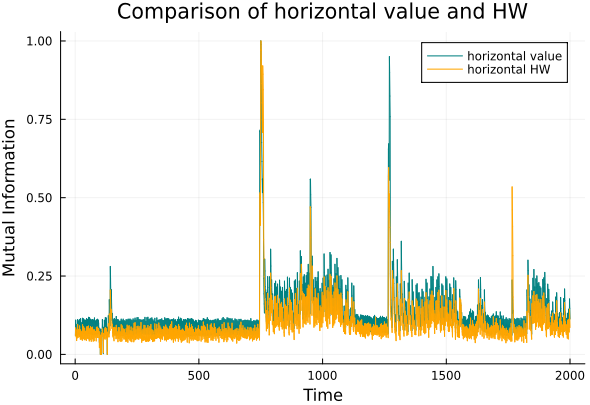
\includegraphics[width=0.8\textwidth]{img_files/horizontal_one_byte}
		\caption{Graphe représentant l'information mutuelle entre la consommation de courant et le poids de Hamming du premier octet de $S_4$ en fonction du temps en bleu et la valeur en orange, pour un nonce fixé}
		\label{hHW&val}
	\end{figure}
	
	\begin{figure}[H]
		\centering
		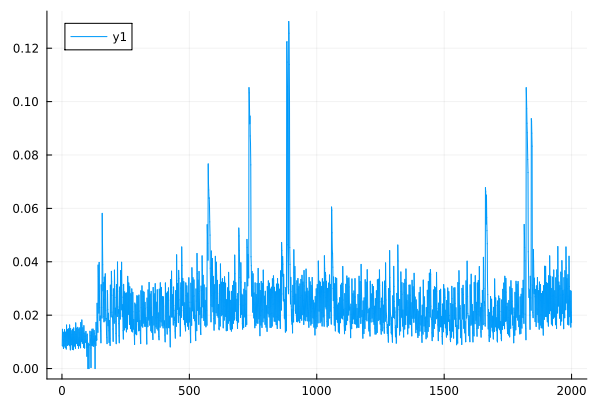
\includegraphics[width=0.8\textwidth]{img_files/hHW_one_byte}
		\caption{Graphe représentant l'information mutuelle entre la consommation de courant et le poids de Hamming du premier octet de $S_4$ en fonction du temps pour des nonces aléatoires}
		\label{hHW1}
	\end{figure}
	
	Dans les graphes \ref{hHW1} et \ref{hHW&val}, on observe des pics qui semblent montrer des points d'intérêts, cependant ils restent tout de même nombreux à nonce aléatoire et l'information mutuelle absolue n'est pas forcément très impressionnante à nonce aléatoire, ce qui n'est pas nécessairement un problème puisqu'on essaie de distinguer déjà le moment d'utilisation de cet octet. Il semble que l'information mutuelle permette ainsi de distinguer les points d'intérêt. De plus, la courbe de valeur étatn un zoom exact de la courbe de poids de Hamming, on reste logique et aucun des deux ne se distinguent particulièrement.
	
	\begin{figure}[H]
		\centering
		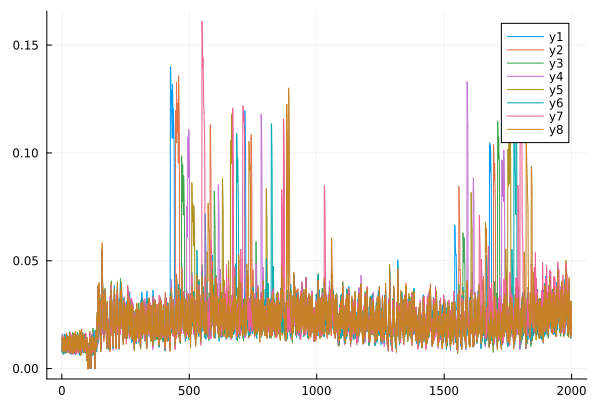
\includegraphics[width=0.65\textwidth]{img_files/hHW_each_byte}
		\caption{Graphe de l'information mutuelle entre la consommation de courant et le poids de Hamming de chacun des 8 octets de $S_4$ en fonction du temps}
		\label{hHW8}
	\end{figure}
	
	\begin{figure}[H]
		\centering
		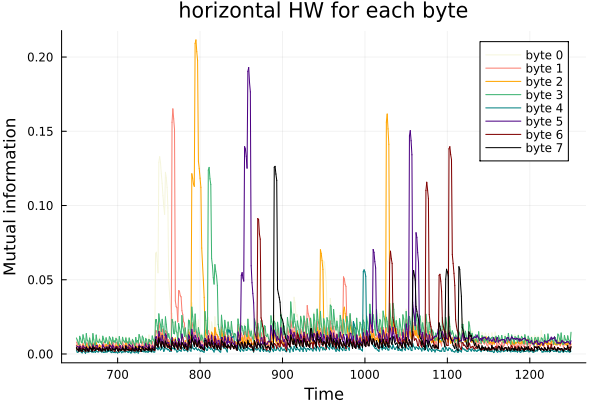
\includegraphics[width = 0.65\textwidth]{img_files/hHW_8_bytes_zoom}
		\caption{Comme le graphe précédent mais pour un nonce fixé et zoomé pour mieux voir}
		\label{hHW8_zoom}
	\end{figure}
	
	Dans le graphe \ref{hHW8}, on observe que les pics de chaque octet semblent environ successifs, ce qui signifierait qe chaque octet est écrit l'un après l'autre dans les registres, ce qui semble cohérent. Cette observation est plus claire dans le graphe \ref{hHW8_zoom}, où on observe également que l'un des octets n'a pas de pics.
	
	\begin{figure}[H]
		\centering
		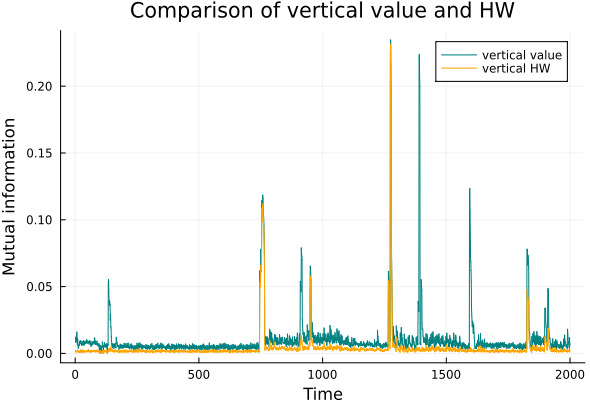
\includegraphics[width=0.8\textwidth]{img_files/vertical_one_bit}
		\caption{Graphe de l'information mutuelle entre la consommation de courant et le poids de Hamming de la concaténation du premier bit de chacun des 5 mots de $S$ en orange et leur valeur en bleu pour un nonce fixé}
		\label{vHW}
	\end{figure}
	
	\begin{figure}[H]
		\centering
		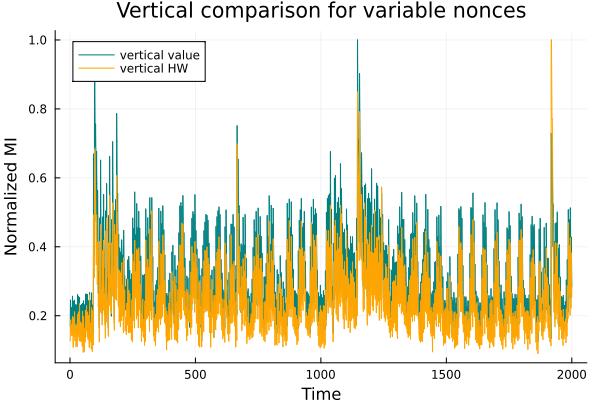
\includegraphics[width=0.8\textwidth]{img_files/vertical_one_byte}
		\caption{Graphe de l'information mutuelle entre la consommation de courant et le poids de Hamming de la concaténation du premier bit de chacun des 5 mots de $S$ en bleu et leur valeur en orange pour des nonces variables}
		\label{vHW&val}
	\end{figure}
	
	Dans les graphes \ref{vHW&val} et \ref{vHW}, on observe qu'il y a également de nombreux pics pour l'hypothèse verticale, légèrement plus nombreux et également que ces pics sont les mêmes en valeur et en poids de Hamming, la valeur absolue de l'information mutuelle est juste plus importante pour la valeur. C'est ainsi assez cohérent. Dans le cas du nonce fixé, il y a plus de pics lorsqu'on regarde la valeur que le poids de Hamming (ce qui est moins cohérent).
	
	\begin{figure}[H]
		\centering
		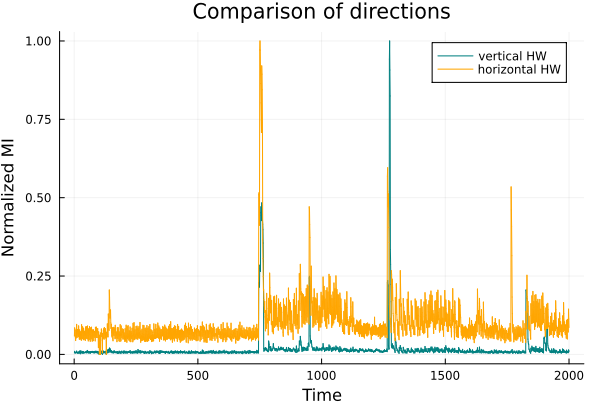
\includegraphics[width=0.8\textwidth]{img_files/h_and_v_one_byte}
		\caption{Graphe de l'information mutuelle entre la consommation et la valeur horizontale en orange et la valeur verticale en bleu}
		\label{hvval}
	\end{figure}
	
	Dans le graphe \ref{hvval}, on observe que les pics d'utilisation horizontale du premier octet de $S_4$ est à peu près simultané avec l'utilisation verticale du premier bit, ce qui parait étonnant. En effet, notre hypothèse était que l'utilisation horizontale était liée à l'écriture et apparaissait donc ultérieurement à l'utilisation verticale liée au calcul.
	
	\begin{figure}[H]
		\centering
		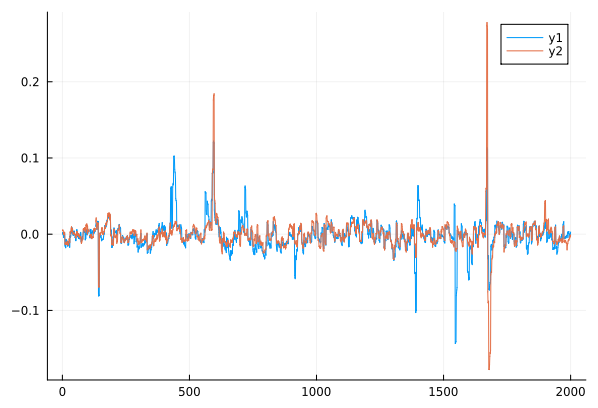
\includegraphics[width=0.8\textwidth]{img_files/vertical_corr}
		\caption{Graphe de la corrélation de Pearson entre la consommation et le poids de Hamming vertical en bleu et la valeur verticale en orange}
		\label{vcor}
	\end{figure}
	
	Dans le graphe \ref{vcor}, on observe que la corrélation de Pearson donne également un plutôt bon résultat, même si la valeur absolue n'est pas très importante, on voit des pics importants à certains moments, cohérents entre valeur et poids de Hamming.
	
	\begin{figure}[H]
		\centering
		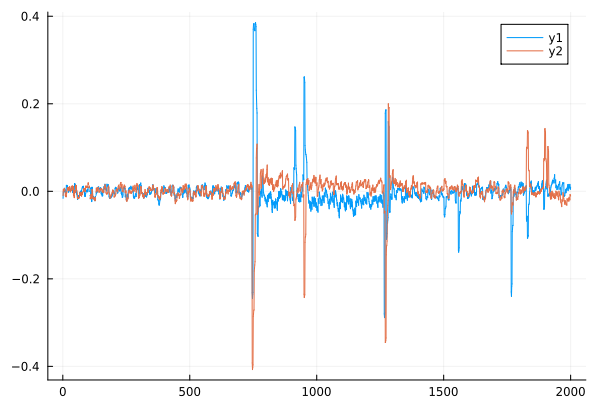
\includegraphics[width=0.8\textwidth]{img_files/horizontal_one_bit_corr}
		\caption{Graphe de la corrélation de Pearson entre la consommation et le poids de Hamming horizontal en bleu et la valeur en orange}
		\label{hcor}
	\end{figure}
	
	Dans le graphe \ref{hcor}, on observe un corrélation de Pearson assez marquée (0.4 en absolu c'est quand même beaucoup), en particulier pour la corrélation avec la valeur qui a des valeurs négatives très importantes (on est supposés trouver une corrélation négative pour la ChipWhisperer.)
	
	\begin{figure}[H]
		\centering
		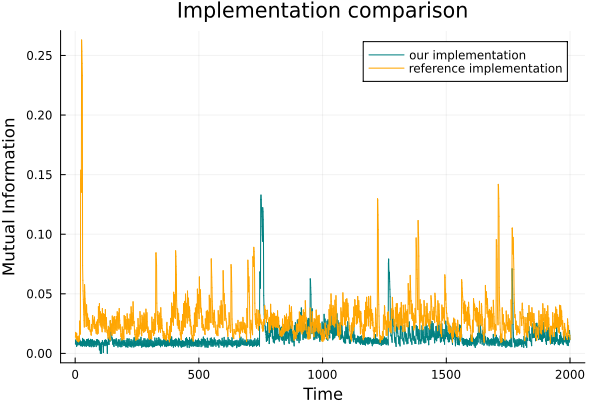
\includegraphics[width=0.8\textwidth]{img_files/comp_ref_hHW}
		\caption{Graphe de l'information mutuelle entre la consommation et le poids de Hamming horizontal en bleu sur l'implémentation de référence et en orange sur notre implémentation}
		\label{compref}
	\end{figure}
	
	Dans le graphe \ref{compref}, on voit qu'on a les mêmes fuites dans l'implémentation de référence donc notre implémentation n'est pas complètement stupide. Par contre ces fuites ne sont pas exactement au même endroit : normal la S-Box n'a pas été écrite exactement pareil. Une idée intéressante serait de peut-être modifier légèrement notre Sbox et faire plein de tests pour voir où exactement ça fuit dans la SBox
	
	\begin{figure}[H]
		\centering
		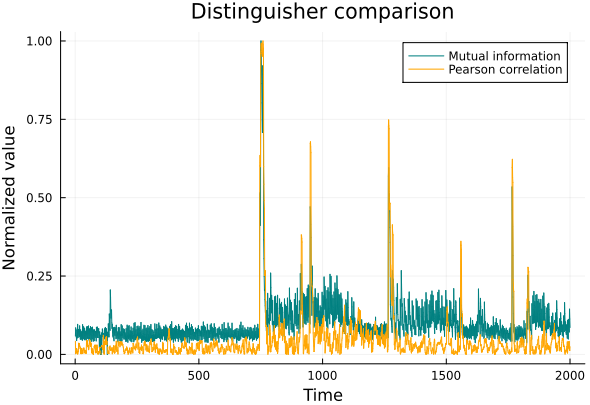
\includegraphics[width=0.8\textwidth]{img_files/corr_vs_MI_hHW}
		\caption{Graphe comparant l'information mutuelle (en orange) et la corrélation de Pearson (en bleu) pour un attaque horizontale sur l'implémentation de référence}
		\label{corvsMI}
	\end{figure}
	
	Dans le graphe \ref{corvsMI}, on voit que les pics sont les mêmes selon le distingueur, ce qui est rassurant, et que les pics sont un peu plus nets pour l'information mutuelle, ce qui peut permettre d'espérer de meilleurs résultats pour une attaque CPA utilisant la MI comme distingueur.
	
	\warning Dans l'implémentation de référence, on renvoie \verb|true| quand ça échoue et pas quand c'est bien intègre. De plus, l'implémentation de référence renvoie le message déchiffré même si le message n'est pas intègre
	
	\subsection{Résumé de séance}
	\begin{itemize}
		\item Analyse des graphes
		\item Adaptation de l'implémentation de référence pour la CW
		\item Capture des traces pour l'implémentation de référence
		\item Comparaison entre l'implémentation de référence et la nôtre (similaire)
	\end{itemize}
	
	\subsection{Objectifs de la séance prochaine}
	\begin{todolist}
		\item[\done] Choisir les meilleurs graphes à ajouter dans le rapport
		\item Enfin finir de corriger l'attaque de Daemen et al.
		\item[\done] Faire l'information mutuelle comme distingueur
	\end{todolist}
	
	
	\section{Séance 20 : 18/06/2025}
	\subsection{Notes de séance}
	Un autre article sur la même analyse que Daemen (\url{https://eprint.iacr.org/2023/1598.pdf}) ne donne pas les mêmes valeurs pour $y_0$
	
	\subsection{Résumé de séance}
	\begin{itemize}
		\item Analyse de certains graphes dans le rapport
		\item Nouvelle capture de traces sur l'implémentation de référence pour Daemen, sans succès
		\item Nombreuses tentatives de debuggage
	\end{itemize}
	
	
	\section{Séance 21 : 19/06/2025}
	\subsection{Notes de séance}
	D'après l'article de Cascade, ça ne sert à rien d'attaquer après la S-box, puisque plusieurs pairs de clés donnent la même réponse pour un bit vertical, mais ça ne veut pas dire que ça ne marche pas pour la concaténation des 5 bits verticaux. En effet, ce ne sont pas les mêmes clés qui fautent pour y0 et y1, donc en considérant les deux, on devrait pouvoir distinguer chacune des deux clés. Cependant, d'après leur analyse, comme les hypothèses de clés restent très corrélées entre elles, il faut beaucoup de traces. 40K n'est visiblement pas suffisant, même sur CW. Ainsi, faire en premier lieu les hypothèses de clés puis en déduire la sortie et faire la corrélation n'est pas une bonne idée. Cependant, d'après l'étude de Sarry, on pourrait grâce à un apprentissage retrouver l'entrée à partir de la sortie, sous condition de pouvoir relancer pour des nonces pratiques. Permettrait en effet de régler le problème.
	
	Mentionnons que certains articles simplifient encore plus les équations que Modou Sarry.
	
	\subsection{Résumé de séance}
	\begin{itemize}
		\item Vérification que l'attaque logique ne marchait pas
		\item Tentative de correction encore et encore c'est que le début d'accord d'accord
		\item Jolification de mon code Ascon
		\item Encore un peu de rapport
	\end{itemize}
	
	
	\section{Séance 22 : 20/06/2025}
	\subsection{Notes de séance}
	\textbf{Réponse aux questions :}
		\begin{itemize}
		\item Vérifier l'analyse des graphes de la séance \ref{s19} afin de pouvoir rédiger les interprétations et conclusions du leak dans le rapport
		\item Dans l'implémentation de référence, à quoi sert le paramètre nsec ? Il est juste utilisé pour \verb|(void) nsec);| au début du chiffrement et du déchiffrement. $\rightarrow$ à rien certainement juste utilisé pour ressembler à la norme
		\item Dans l'implémentation de référence, on inclut un fichier qui n'existe pas (agaçant, mais facile à réécrire) et on déchiffre peu importe l'intégrité, c'est un peu problématique, non ? $\rightarrow$ pas grave
		\item Est-ce que mon déchiffrement du tag est sensible aux attaques "time-based" ? Parce que la façon de l'implémenter pour la référence est super compliquée (peut-être problème avec "==" ?) $\rightarrow$ en effet, ce n'est pas nécessairement la même durée, d'autant plus avec certaines options de compilation (\verb|-Ofast| peut décider de sauter une partie de ma boucle), mais d'un autre côté ce n'est pas grave pour mon implémentation
		\item Comment utiliser les équations ? Si on a qu'une seule trace, nécessité d'avoir eu une phase d'apprentissage avant, car on ne peut en déterminer des statistiques, si on en a plusieurs, on ne peut pas retrouver $S_4$ car chaque trace a un $S_4$ différent dépendant du nonce $\rightarrow$ on va attaquer à nonce fixé le déchiffrement
	\end{itemize}
	
	\noindent Lors du déchiffrement, c'est l'attaquant qui fournit le nonce, le tag, etc... et peu importe si ce n'est pas cohérent avec l'intégrité, puisque la phase attaquée est la phase de déchiffrement. Ainsi, l'objectif est par attaque CPA dont les hypothèses sont les 5-bits de la sortie de la S-box $S_0,S_1,S_2,S_3,S_4$ d'avec l'information mutuelle verticale au poids de Hamming réussir à retrouver la bonne sortie, puis relier cette sortie à la clé à partir du tableau de Sarry.
	
	
	\subsection{Résumé de séance}
	\begin{itemize}
		\item Bilan hebdomadaire
		\item Rédaction du concept de la nouvelle attaque
		\item Conférence de sécurité sur Ascon
		\item Création d'un github pour ne pas perdre toutes mes données
	\end{itemize}
	
	\subsection{Objectifs de la séance prochaine}
	\begin{todolist}
		\item[\done] Nouveau main
		\item[\done] Nouveau python
		\item[\done] Nouvelle capture
		\item[\done] Nouvelle analyse
		\item[\done] Interprétation des résultats
	\end{todolist}
	
	\section{Séance 23 : 23/06/2025}
	\subsection{Notes de séance}
	Problème: toutes les clés avec le même poids de Hamming vont être autant corrélées à la consommation de courant, car on n'a pas de diffusion éloignant les hypothèses proches et tous les appels ne donnent pas vraiment de statistique puisqu'on y retrouve exactement la même sortie : voir si on peut faire une corrélation par valeur qui serait peut-être un peu mieux.
	
	\noindent Voir sur le carnet l'autre idée. Très semblable à l'attaque normale, donc ne va certainement pas très bien marcher.
	
	\subsection{Résumé de séance}
	\begin{itemize}
		\item Nouveau main qui appelle le déchiffrement
		\item Nouvelle capture
		\item Idée principale ne fonctionnant pas, élaboration d'une nouvelle idée d'attaque
	\end{itemize}
	
	\subsection{Objectifs de la séance prochaine}
	\begin{todolist}
		\item[\done] Finir l'autre attaque
	\end{todolist}
	
	
	\section{Séance 24 : 24/06/2025}
	\subsection{Notes de séance}
	Ce n'est pas vraiment fameux, les pics sont au même endroit pour toutes les hypothèses de clé... Quand on augment le nombre de traces, le point d'intérêt est plus net, mais chaque hypothèse donne le même résultat...
	
	\noindent Voir le carnet pour les notes de séance
	
	\noindent \textbf{Remarque :} il faudrait relire bien l'article de Cascade pour s'assurer que l'attaque ne marche pas non plus pour les mêmes raisons
	
	Au pire, si on ne trouve pas de solution, on peut se rassurer et se dire que le fait qu'on soit capable de choisir le nonce au déchiffrement ne rend pas l'attaque plus facile contrairement à ce que je pensais
	
	\subsection{Résumé de séance}
	\begin{itemize}
		\item Implémentation de l'attaque à nonce plus ou moins fixé
		\item Essais de plusieurs quantité de nonce
		\item Compréhension des traces
	\end{itemize}
	
	\subsection{Objectifs de la séance prochaine}
	\begin{todolist}
		\item[\done] Comprendre le problème évoqué dans le carnet $\rightarrow$ on n'a pas assez de valeurs de nonces possibles, doc les variations sont les mêmes partout
		\item[\done] \'Etudier la réponse d'Hélène 
		\item[\done] Trouver une autre idée d'attaque ou une preuve se raccrochant à l'article de Cascade pour voir que même en pouvant choisir son nonce, on est embêté $\rightarrow$ j'ai vraiment l'impression que c'est exactement la même attaque
		\item[\done] Voir si en choisissant des nonces plus aléatoires, donc qui ne respectent pas nécessairement les équations de Modou pour chaque nonce, ça marche mieux (pas l'air si on réfléchit rapidement)
	\end{todolist}
	
	
	\section{Séance 25 : 25/06/2025}
	\subsection{Notes de séance}
	À l'air de marcher beaucoup mieux lorsque le nonce est complètement aléatoire, donc on peut de nouveau se dire qu'on attaque le chiffrement.
	
	\noindent Malheureusement, les clés misent en avant ne semblent pas être très prometteuses.
	
	\noindent On est vraiment revenues à l'attaque de base j'ai l'impression...
	
	\noindent Plus je travaille dessus, plus j'ai l'impression qu'il n'y a pas d'attaque CPA simple sur la S-box, il faut vraiment que je réussisse celle de Daemen sur la permutation
	
	\subsection{Résumé de séance}
	\begin{itemize}
		\item Passage à des nonces complètement aléatoires
		\item Capture de plus de traces pour réessayer avec plus de données
	\end{itemize}
	
	\subsection{Objectifs de la séance prochaine}
	\begin{todolist}
		\item[\done] Rendez-vous avec Hélène
		\item[\done] Commencer présentation
	\end{todolist}
	
	
	\section{Séance 26 : 26/06/2025}
	\subsection{Notes de séance}
	On arrive à la conclusion que le pic n'est pas du tout un bon pic mais plutôt un point d'activité du circuit qui n'a aucun lien avec la bonne clé.
	
	L'idée principale de l'attaque paraît tout de même bien, ie de faire les hypothèses sur la sortie puis de regarder le lien avec la consommation, puis remonter en arrière.
	
	\c{C}a ne résout pas tous les problèmes, mais comme test intéressant : pour un HW fixé (et pratique, 0 et 5 pas fou par exemple e.g. 3), trouver tous les antécédents, et faire les test pour ces antécédents là et pour d'autres et pour le mix et voir si on a une meilleure corrélation comme attendu entre 3 et la consommation. Si ça ne marche pas, on peut aussi regarder le lien avec la distance de Hamming entre l'entrée et la sortie, ou la valeur (mais c'est ce que j'ai fait et ça n'a pas trop l'air de fonctionner)
	
	\textbf{Réponses aux questions :}
	\begin{itemize}
		\item Finalement on revient de plus en plus à l'attaque de base qui ne fonctionne pas de la même façon... $\rightarrow$ vaiation si on fait l'hypothèse directement sur le poids de Hamming
		\item Les pics que je vois à chaque sbox vertical sont simultanés, est-ce que c'est logique ? $\rightarrow$ regarder dans \verb|Autres mesures|, pas vraiment puisque là-bas les pics sont successifs également... Sous-entend que ce qu'on voit ce ne sont pas vraiment les pics voulus ?
	\end{itemize}
	
	\subsection{Résumé de séance}
	\begin{itemize}
		\item Présentation
		\item Rendez-vous avec Hélène
		\item Relecture du rapport
	\end{itemize}
	
	\subsection{Objectifs de la séance prochaine}
	\begin{todolist}
		\item[\done] Relire rapport
		\item[\done] Envoyer le rapport
		\item[\done] Continuer/finir diaporama
		\item[\done] Envoyer diaporama
		\item[\done] Essayer attaque discutée (voir notes de cours du jour)
	\end{todolist}
	
	
	\section{Séance 27 : 27/06/2025}
	\subsection{Notes de séance}
	Problèmes informatiques et visite, donc rien de concret...
	
	\section{Séance 28: 30/06/2025}
	\subsection{Notes de séance}
	On voit bien que le poids de Hamming fuite bien, car lorsqu'on compare les bons poids par rapport à des poids aléatoires, l'un a des points d'intérêt et pas l'autre. Voir le graphe suivant:
	
	\begin{figure}[H]
		\centering
		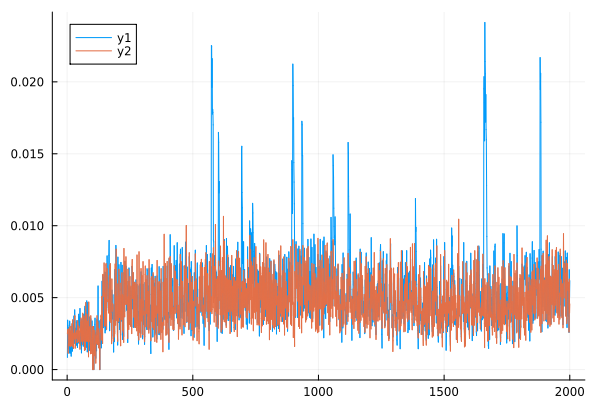
\includegraphics[scale=0.8]{img_files/HWvrai_vs_HWalea}
		\caption{Information mutuelle entre la consommation et les vrais poids de Hamming en bleu et entre la consommation et des valeurs aléatoires en orange}
	\end{figure}
	
	Le problème étant que ça voudrait dire que notre attaque devrait au moins marcher un peu...
	
	\subsection{Résumé de séance}
	\begin{itemize}
		\item Finission du diaporama et envoi du diaporama et rapport
		\item Visite du LHS
		\item Vérification de la fuite du poids de Hamming
	\end{itemize}
	
	\subsection{Objectifs de la séance prochaine}
	\begin{todolist}
		\item[\done] Trouver une idée de quoi en faire maintenant qu'on sait que le poids de Hamming fuit bien
		\item[\done] Réessayer l'expérience des HW, sauf que cette fois on ne choisit pas d'antécédent particulier, juste on regarde ce qui pique le mieux entre des HW aléatoiers et les vrais
		\item[\done] Relire à tête reposée l'attaque DPA, une dernière fois
		\item[\done] Refaire les graphes avec un légende (si possible plus clairs)
		\item[\done] Répondre au mail pour la présentation
	\end{todolist}
	
	
	\section{Séance 29 : 1/07/2025}
	\subsection{Notes de séance}
	Maintenant qu'on sait que le poids de Hamming fuit bien, on arrive à la conclusion que si on prend une mauvaise hypothèse, puisque la s-box est suppozée avoir un comportement aléatoire, alors le HW de sortie est random et ne devrait pas piquer. En revanche, si c'est le bon Hamming Weight, ça ne devrait pas piquer.
	
	\noindent \textbf{Observatins :} De manière très intéressante, on voit bien qu'il y a des points d'intérêts si ce sont les bons HW et il n'y en a pas si ce sont des HW aléatoires. De plus, tous les HW d'un même octet ont des points d'intérêts simultanés, mais pour plusieurs octets, c'est sucessif. Est-ce que tous lse calculs verticaux d'un même octet sont simultanés ? Lorsqu'on a des clés et nonces parfaitement aléatoires, on peut distinguer les vrais sorties de sorties aléatoires grâce à leu poids de Hamming.
	
	\noindent Assez étonnament, quand c'est la clé qu'on fait varier, l'hypothèse fausse est très proche derrière...
	
	\subsection{Résumé de séance}
	\begin{itemize}
		\item Différents exemples pour comparer des faux poids de Hamming avec les vrais
		\item Maintenant comparer les vrais poids de Hamming pour les fausses clés : i.e. comme avant pour deux clés et on regarde la corrélation avec la bonne clé ou avec la mauvaise
	\end{itemize}
	
	\subsection{Objectifs de la séance prochaine}
	\begin{todolist}
		\item[\done] Refaire les graphes
		\item[\done] Répondre au mail
		\item[\done] Corriger la présentation
		\item[\done] Réfléchir à pourquoi la fausse clé donne une bonne corrélation : la s-box devrait disperser
	\end{todolist}
	
	
	\section{Séance 31 : 3/07/2025}
	\subsection{Notes de séance}
	Il y a une forte corrélation entre les clés fausses et juste car lorsqu'on prend une hypothèse de clé fixe, les sortie ne sont pas réellement aléatoire. Cependant, surbeaucoup de traces, on devrait quand-même pouvoir distinguer la bonne clé.
	
	\noindent Ce n'est pas très concluant: même de fausses hypothèses pointent des fois, c'est un peu le hasard...
	
	\noindent \c{C}a ne marchera probablement pas 
	
	\subsection{Résumé de séance}
	\begin{itemize}
		\item Graphe avec titre et couleur pour échelle de gris
		\item Calcul pour une fausse clé sur beaucoup de traces pour voir si on peut distinguer une fausse clé d'une vraie clé
		\item Calcul d'images
		\item Entraînement à la présentation
	\end{itemize}
	
	\subsection{Objectifs de la séance prochaine}
	\begin{todolist}
		\item[\done] Rendez-vous hebdomadaire : parler que l'attaque ne marchera certainement pas, même si les HW fuit, chaque clé donne des hypothèses trop proches
	\end{todolist}
	
	
	\section{Séance 32 : 4/07/2025}
	\subsection{Notes de séance}
	\textbf{Remarques sur la présentation :} 
	\begin{todolist}
		\item[\done] Ajouter encadrant, équipe, date
		\item[\done] Slides doivent être redondantes
		\item[\done] Ne pas présenter les autres étapes de la permutation
		\item[\done] Revoir l'ordre : Intro avant le plan -> très général, pas balancer Ascon d'un coup, puis Ascon -> la permutation linéaire juste les évoquer, expliquer le state et l'initialisation, puis tableau équations puis CW (sans parler de triggers) puis évoquer CPA plus simplement et sans exemple
		\item[\done] Revendre une meilleure conclusion, peut-être rajouter une slide d'explication de pourquoi ça ne marche pas
		\item[\done] Refaire les slides
		\item[\done] Rajouter les citations des figures
		\item[\done] Rajouter les annexes
	\end{todolist}
	
	\noindent \textbf{Remarques sur le rapport :} 
	\begin{todolist}
		\item[\done] Enlever "nous"
		\item[\done] Enlever futurs
		\item[\done] Réécrire l'introduction selon un modèle (motivations, apports, plan, ...)
		\item[\done] Ajouter de meilleures figures
		\item[\done] Ajouter les citations des figures
		\item[\done] Ajouter l'équipe
		\item[\done] Enlever le tableau
		\item[\done] Ajouter le code en annexe
		\item[\done] Expliquer plus en détail Ascon
		\item[\done] Revoir les annexes (ne pas mettre les équations en annexe, surtout pour les étapes de permutation, mettre un tableau d'abréviation, peut-être y mettre des graphes moins utiles à nonces variables par exemple)
		\item[\done] S'assurer que les figures soient au bon endroit(avec [h!])
		\item[\done] Ajouter le citation CPA
		\item[\done] Vérification de format
		\item[\done] Relecture complète (ajout dans les résultats du fait que les HW aléatoires marchent avec un graphe en annexe)
		\item[\done] Vérification orthographe/grammaire
		\item[\done] Si temps supplémentaire : refaire légende du graphe normalisé/meilleures couleurs pour les 8 octets ?
		\item[\done] faire la s-Box en Tikz, 
		\item[\done] Refaire le Tikz du déchiffrement pour être cohérent sur le code couleur
	\end{todolist}
	
	\noindent \textbf{Réponse à la question :}
	\begin{itemize}
		\item Comment ça se fait que pour des faux HW, on ait une IM négligeable, mais que pour des fausses clés, supposées donc donner des HW aléatoires par hypothèse crypto, on ait une corrélation ? $\rightarrow$ voir le carnet, pas assez de variations quand on a une clé fixée...
	\end{itemize}
	
	\noindent \textbf{Réunion Ascon :} Repousser la cyclicité dans Exact Soft Analytical SCA using Tractable Circuits, faire du BP en gros, c'est compliqué mais bon résultat
	
	\subsection{Résumé de séance}
	\begin{itemize}
		\item Rendez-vous hebdomadaire
		\item Correction du rapport
		\item Réunion Ascon
	\end{itemize}
	
	\subsection{Objectifs de la séance prochaine}
	\begin{todolist}
		\item Regarder comment protéger Ascon
		\item[\done] Corriger rapport
		\item[\done] Corriger présentation
	\end{todolist}
	
	
	\section{Séance 33 : 7/07/2025}
	\subsection{Notes de séance}
	\textbf{Parties supprimées du rapport :}
	
	If the permutation is applied $a$ times, the constant for the round $i$ is \verb|const|$_{16-a+i}$ in table \ref{consts}.\\
	If it is applied $b$ times, then \verb|const|$_{16-b+i}$ 
	
	\begin{figure}[h]
		\centering
		\footnotesize
		\begin{tabularx}{0.5\textwidth}{cc||cc}
			\hline
			$i$&\verb|const|$_i$&$i$&\verb|const|$_i$\\
			\hline
			0&\verb|0x000000000000003c|&8&\verb|0x00000000000000b4|\\
			1&\verb|0x000000000000002d|&9&\verb|0x00000000000000a5|\\
			2&\verb|0x000000000000001e|&10&\verb|0x0000000000000096|\\
			3&\verb|0x000000000000000f|&11&\verb|0x0000000000000087|\\
			4&\verb|0x00000000000000f0|&12&\verb|0x0000000000000078|\\
			5&\verb|0x00000000000000e1|&13&\verb|0x0000000000000069|\\
			6&\verb|0x00000000000000d2|&14&\verb|0x000000000000005a|\\
			7&\verb|0x00000000000000c1|&15&\verb|0x000000000000004b|\\
			\hline
		\end{tabularx}
		\caption{Constant-addition layer, each box representing a byte of one of the 64-bit words{}}
		\label{consts}
	\end{figure} 	
	
	
	with the S-box the lookup table \ref{lookup_sbox}.
	
	\begin{figure}[h]
		\small
		\centering
		\begin{tabular}{|c||*{8}{c|}}
			\hline
			$x$&0&1&2&3&4&5&6&7\\
			\hline
			$S-box(x)$&4&b&1f&14&1a&15&9&2\\
			\hline\hline
			$x$&8&9&a&b&c&d&e&f\\
			\hline
			$S-box(x)$&1b&5&8&12&1d&3&6&1c\\
			\hline\hline
			$x$&10&11&12&13&14&15&16&17\\
			\hline
			$S-box(x)$&1e&13&7&e&0&d&11&18\\
			\hline\hline
			$x$&18&19&1a&1b&1c&1d&1e&1f\\
			\hline
			$S-box(x)$&10&c&1&19&16&a&f&17\\
			\hline
		\end{tabular}
		\caption{Lookup table for the 5-bit S-box}
		\label{lookup_sbox}
	\end{figure}
	
	It can also be computed using the circuit \ref{circuit_sbox}, which gives the equations \ref{equations_sbox}.
	
	
	
	\begin{figure}[H]
		\centering
		\begin{lstlisting}[style=CStyle]
			state[0] ^= state[4];
			state[4] ^= state[3];
			state[2] ^= state[1];
			uint64_t t0 = ~state[0];
			uint64_t t1 = ~state[1];
			uint64_t t2 = ~state[2];
			uint64_t t3 = ~state[3];
			uint64_t t4 = ~state[4];
			t0 &= state[1];
			t1 &= state[2];
			t2 &= state[3];
			t3 &= state[4];
			t4 &= state[0];
			state[0] ^= t1
			; state[1] ^= t2;
			state[2] ^= t3;
			state[3] ^= t4;
			state[4] ^= t0;
			state[1] ^= state[0];
			state[0] ^= state[4];
			state[3] ^= state[2];
			state[2] =~ state[2];
		\end{lstlisting}
		\caption{Equations to compute the S-box}
		\label{equations_sbox}
	\end{figure}
	
	It provides diffusion throughout each word $S_i \leftarrow \Sigma_i(S_i)$:
	
	\begin{gather*}
		\Sigma_0(S_0) = S_0 \oplus (S_0 >>> 19) \oplus (S_0 >>> 28)\\
		\Sigma_1(S_1) = S_1 \oplus (S_1 >>> 61) \oplus (S_1 >>> 39)\\
		\Sigma_2(S_2) = S_2 \oplus (S_2 >>> \;  1) \oplus (S_2 >>> \; 6)\\
		\Sigma_3(S_3) = S_3 \oplus (S_3 >>> 10) \oplus (S_3 >>> 17)\\
		\Sigma_4(S_4) = S_4 \oplus (S_4 >>> \; 7) \oplus (S_4 >>> 41)\\
	\end{gather*}
	
			
	\begin{figure}[h]
		\centering
		\begin{tabularx}{0.4\textwidth}{|*{8}{>{\centering\arraybackslash}X|}>{\centering\arraybackslash}X}
			\cline{1-8}
			&&&&&&&&$S_0$\\
			\cline{1-8}
			&&&&&&&&$S_1$\\
			\cline{1-8}
			&&&&&&& \LARGE $\oplus$&$S_2$\\
			\cline{1-8}
			&&&&&&&&$S_3$\\
			\cline{1-8}
			&&&&&&&&$S_4$\\
			\cline{1-8}
		\end{tabularx}
		\caption{Constant-addition layer, each box representing a byte of one of the 64-bit words{}}
		\label{const_lay}
	\end{figure} 
	
	\subsection{Résumé de séance}
	\begin{itemize}
		\item Envoi du mail
		\item Continuation de la correction du rapport
	\end{itemize}
	
	\subsection{Objectifs de la prochaine séance}
	\begin{todolist}
		\item[\done] Finaliser correction du rapport
		\item[\done] Correction de la présentation
	\end{todolist}
	
	
	\section{Séance 34 : 8/07/2025}
	\subsection{Notes de séance}
	Extraits de la présentation supprimés :
	
%	\begin{frame}
%		\frametitle{Steps for a CPA attack}
%		
%		\begin{columns}[T]
%			\column{0.32\textwidth}
			\textbf{Campaign:}\\
			Choose:
			\begin{itemize}
				\item target $k$
				\item attack path $\mathcal{R}(k,O_S)=O_R$
			\end{itemize}
			Compute the algorithm multiple times to gain \textbf{traces}
			
%			\column{0.32\textwidth}
			\textbf{Prediction:}\\
			Find a model for $\mathcal{R}$, $\mathcal{R}_m(k,O_S) = P_{m,k}$
			
%			\column{0.32\textwidth}
			\textbf{Confrontation:}\\
			Choose a distinguisher for each hypothesis $k$, confronting $O_R$ and $P_{m,k}$\\
			Finds the best hypothesis $k_d$
%		\end{columns}
%	\end{frame}
	
	\subsubsection{Basic example on AES}
	%\begin{frame}
	%	\frametitle{Example on AES}
		
	%	\begin{columns}[T]
	%		\column{0.32\textwidth}
			\textbf{Campaign:}\\
			\begin{itemize}
				\item $k = $ one byte of the secret key $K_0$
				\item $O_R = $ power consumption during the S-box
				\item $O_S = p$ one byte of the plaintext $T$
			\end{itemize}
			
	%		\column{0.32\textwidth}
			\textbf{Prediction:}\\
			$\mathcal{R}_m(k,p) = HW(S-box(p \oplus k))$
%			\begin{figure}
%				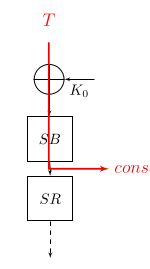
\includegraphics[width=0.5\textwidth]{attack_path_aes}
%				\caption{Attack path on AES}
%			\end{figure}
			
	%		\column{0.32\textwidth}
			\textbf{Confrontation:}\\
			Distinguisher: Pearson correlation
			\begin{figure}[H]
				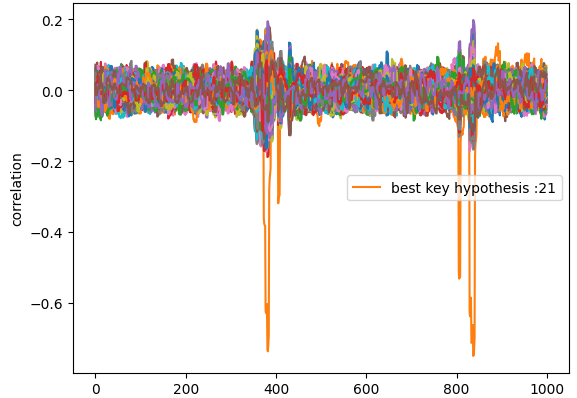
\includegraphics[width=\textwidth]{img_files/corr_aes}
				\caption{Correlation for each key hypothesis with the power consumption}
			\end{figure}
	%	\end{columns}
	%\end{frame}
	
	\begin{itemize}
		\item Initialization: state creation and modification
		$$S \leftarrow p^{a}( \underbrace{IV}_{S_0}||\underbrace{K}_{S_1,S_2}||\underbrace{n}_{S_3,S_4})$$
		$$S \leftarrow S \oplus 0^{192} || K$$
		\item Associated data process: updates the state using blocks of $r$-bits from $A=(A_1||..||A_s)$
		\item Plaintext/Ciphertext process: each block of the plaintext or ciphertext is included in the state
		\item Finalization: computes the tag thanks to the key and the state
	\end{itemize}	
	
	\subsection{Résumé de séance}
	\begin{itemize}
		\item Finission des corrections du rapport
		\item Calcul d'une image supplémentaire
		\item Début de correction de la présentation
	\end{itemize}
	
	\subsection{Objectifs de la séance prochaine}
	\begin{todolist}
		\item[\done] Finir présentation
		\item[\done] Passer et se chronométrer
		\item[\done] Regarder combien d'erreur le tag d'Ascon remarque $\rightarrow$ fasse question, problème de l'intégrité pas du code correcteur d'erreurs
		\item[\done] Envoyer présentation par mail pour jeudi
		\item[\done] Envoyer tout à Hélène pour qu'elle puisse relire
	\end{todolist}
	
	
	\section{Séance 35 : 9/07/2025}
	\subsection{Notes de séance}
	Premier passage : 12min47s\\
	Deuxième passage : 11min48s\\
	Troisième passage : 11min50s\\
	Quatrième passage : 11min25s\\
	Cinquième passage : 11min25s\\
	Sixième passage : 10min02s\\
	
	\subsection{Résumé de séance}
	\begin{itemize}
		\item Finissions de la présentation
		\item Chronométrage
		\item Petites modifications supplémentaires du rapport
	\end{itemize}
	
	
	\section{Séance 36 : 10/07/2025}
	\subsection{Notes de séance}
	Septième passage : 10min50s\\
	Huitième passage : 10min40s\\
	
	\section{Séance 37 : 11/07/2025}
	\subsection{Notes de séance}
	Pour projet M1 :
	Damien Marion, IRISA, Hélène Le Bouder, Thomas Rockiki, Ruben
	
	\subsection{À faire aujourd'hui}	
	\begin{todolist}
		\item[\done] ajouter IMT-Atlantique et ENS Rennes sur rapport et présentation
		\item Rendre badge
		\item Ramener matériel
		\item[\done] Récupérer cours ARC
		\item[\done] Faire signer papier de fin de stage
		\item Envoyer retour signé à l'assistante de département
		\item Tout mettre sur le git
		\item Mettre le git en public (au moins implem)
		\item[\done] Ajouter mon nom sur mes codes
		\item[\done] Refaire/Supprimer la slide CPA (Juste mettre traces Ascon, ne pas mettre de slide CPA ni AES)
		\item[\done] Ajouter abréviation AES
		\item[\done] Ajouter référence pour les abréviations
		\item[\done] Envoyer mail Hélène dernière version du rapport et lien vers le git
		\item[\done] Passe de ponctuation pour la présentation (maj et points)
		\item[\done] Vérifier la cohérence des notations sur les slides
		\item Refaire la présentation avec les modifs suivantes : insister sur le côté matériel ans l'intro, plus vite sur le plan, dire le mot confidentialité où on ajoute de l'intégrité, nonce pas forcément aléatoire, citer Modou directement, ne pas dire pourquoi CW, moins déprime dans la voix
		\item[\done] Mettre la référence à la fin pour M. Eichleseder
		\item[\done] Ligne Latex pour faire disparaitre trucs bizarres
	\end{todolist}
	
	
	
	\section{Questions pour l'entretien hebdomadaire}



\end{document}